\documentclass[12pt]{article}
% \textwidth 15.5cm \oddsidemargin 0cm \topmargin -2cm \textheight
% 24cm \footskip 1cm
\usepackage[british]{babel}
\usepackage{epsfig}
\usepackage{amsmath,graphicx,psfrag,pstricks,float,amssymb,fancyhdr,pdfpages, hyperref, enumitem, listings, subfig, diagbox, appendix, lastpage, bm, graphicx}
\usepackage[backend=biber, sorting=none]{biblatex}
% \usepackage[sorting=none]{biblatex}
\usepackage[margin=25mm]{geometry}
%\usepackage{minted}

\DeclareMathOperator*{\argmax}{argmax}
\DeclareMathOperator*{\argmin}{argmin}

% \pagestyle{fancy}
% \pagenumbering{arabic}
% \fancyhead[L]{}
% \cfoot{\thepage}
\fancypagestyle{technical_abstract}{
  \fancyhf{}
  \fancyfoot[C]{Page \thepage}
}

\fancypagestyle{default}{
  \fancyhf{}
  \fancyfoot[C]{Page \thepage\ of \pageref{LastPage}}
}

\pagestyle{fancy}

% \setlength{\headheight}{15pt}
\renewcommand{\headrulewidth}{0pt}
\linespread{1.3}  % "One-and-a-half" spacing

\def\n{\noindent}
\def\u{\underline}
\def\hs{\hspace}
\newcommand{\thrfor}{.^{\displaystyle .} .}
%\newcommand{\bvec}[1]{{\bf #1}}

\addbibresource{bibliography.bib}

\begin{document}

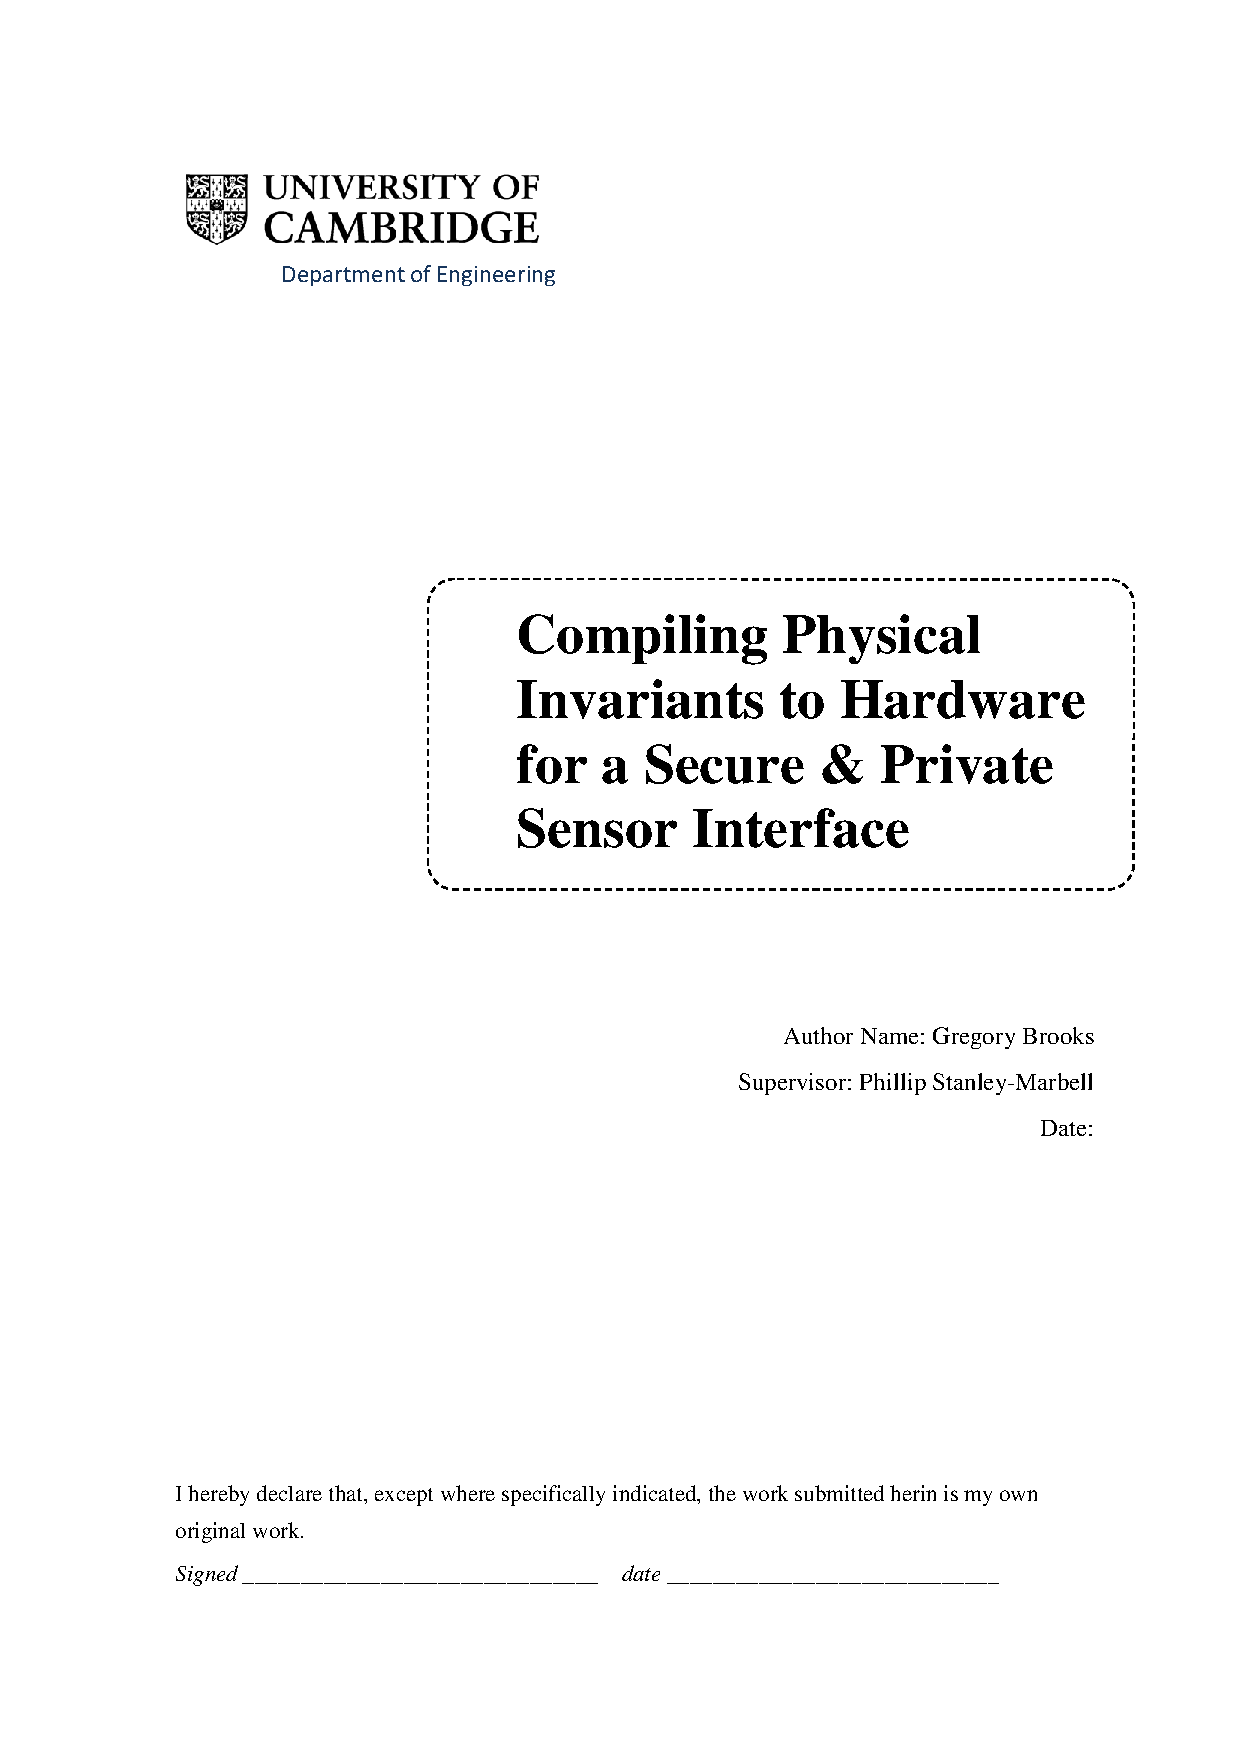
\includepdf[pages={1}]{coversheet.pdf}
\clearpage \mbox{}
\pagenumbering{gobble}
\clearpage
\pagenumbering{arabic}

\noindent

%
% TITLE & CONTENTS PAGE
%

\title
{
  IIB Project Report:\\
  Compiling Physical Invariants to Hardware for a Secure \& Private Sensor Interface\\
}
\author{Gregory Brooks, gb510, Christ's College}
\date{29 May 2019}
\maketitle

\tableofcontents

\pagenumbering{gobble}
\clearpage
\pagenumbering{arabic}

%
% TECHNICAL ABSTRACT
%
\pagestyle{technical_abstract}
\section{Technical Abstract}

\begin{center}
{
  \bf Compiling Physical Invariants to Hardware for a Secure \& Private Sensor Interface\\
}
Gregory Brooks, gb510, Christ's College
\end{center}
\rule{15.7cm}{0.5mm}
\vspace{1cm}

\textit{$\langle$ TODO: write this last$\rangle$}

This project investigates the idea of using the Newton~\cite{Newton} physics description language as part of a multi-sensor embedded local differential privacy system implemented on an iCE40 FPGA.
\textit{$\langle$ TODO: tidy up the above and expand on it if necessary$\rangle$}

\subsection{System Specification}
  \textit{$\langle$ TODO: move to technical abstract?$\rangle$}

  %
  % SYSTEM DIAGRAM
  %

  \subsection{System Diagram}
    \textit{$\langle$ TODO: insert block diagram of system and describe which parts have been the focus of this project$\rangle$}


\newpage


\pagestyle{default}
%
% INTRODUCTION
%

\section{Introduction and Background}
  \subsection{Differential Privacy} \label{intro_diff_priv}
    \textit{Differential privacy} can be thought of as a constraint applied to queries for information from a database whereby information about individual members of the database is obscured whilst still releasing useful aggregate information about a population/demographic as a whole. A simple method of implementing this would be the addition of zero mean noise to database entries --- whilst the noise would obscure the \textit{true} value of individual data points, the mean value of the dataset would remain intact. More formally, \textit{$\epsilon$-differential privacy} is defined by Dwork and Smith~\cite{dwork2010differential} as follows:\\
    \\
    ``A randomized function K gives \textit{$\epsilon$-differential privacy} if for all data sets $x$ and $x'$ differing on at most one element, and all $S \subseteq Range(K)$,
    \begin{equation}
      Pr[K(x) \in S] \leq exp(\epsilon) \times Pr[K(x') \in S],
    \end{equation}
    where the probability space in each case is over the coin flips of the mechanism K.''\\

    Throughout this project, the chosen randomised function K is the Laplace mechanism i.e. the addition of zero mean Laplace distributed random noise to \textit{private} data such as a measurement from a sensor\footnote{The \textit{databases} in this scenario are simply single sensor measurements hence any two \textit{databases} will always differ by at most a single element.} to produce a \textit{noised output} that can be released to untrusted observers (the outside world). This technique provides privacy by ensuring that every possible measurement value (i.e. any value within the sensor measurement range) has a similar posterior probability of being the \textit{true private} value given the observed \textit{noised output}. An outside observer can use the \textit{noised output} to estimate the value of \textit{private} data with some uncertainty but should never be able to deduce it with complete certainty.\\

    The Laplace distribution used by this method has parameter $\frac{\lambda}{\epsilon}$. $\lambda$ refers to the \textit{global sensitivity} of the database query function; in this scenario this is simply the maximum difference between possible sensor measurements i.e. a sensor's measurement range. $\epsilon$ is a privacy scaling parameter, where a smaller $\epsilon$ value results in greater privacy by applying noise with a greater variance, thereby reducing the amount of information each \textit{noised output} value reveals about the \textit{private} data. For a particular application, deciding on an $\epsilon$ value is a tradeoff between utility and privacy since, in the limiting case, an $\epsilon$ value of zero means that the system outputs no useful information (just random noise), consequently keeping the \textit{private} data completely private.\\

    Within the context of embedded electronic systems, recent work (for example, this project builds heavily on the work of Choi et al.~\cite{Choi2018GuaranteeingLD}) has investigated the implementation of differential privacy techniques on low power hardware such as the processors found in smartphones and Internet-of-Things devices. In contrast to the conventional differential privacy model, where a trusted database stores \textit{private} data collected from local hardware, a local differential privacy architecture involves \textit{private} data being masked at the source (e.g. an embedded sensor system) before being sent to an untrusted database~\cite{Kairouz:2014}. This local approach can result in a more secure system since \textit{private} data does not need to be recorded anywhere nor transmitted from local hardware to a remote server.\\

    One of the key advantages of generating random noise with known parameters is that it allows a quantitative \textit{privacy loss}~\cite{Choi2018GuaranteeingLD} to be calculated for each piece of information revealed to the outside world (e.g. with the release of each \textit{noised output} value). Privacy losses can be deducted from a total \textit{privacy budget} allocation --- once the budget has been depleted, a differential privacy system will not release further information to the outside world. An intuitive justification for such a system comes from the fact that if an attacker were allowed to obtain an unlimited number of noised values, they would be able to take the mean of these responses to gain an arbitrarily accurate estimate for the private data value being masked by zero-mean random noise.\\

    One challenge associated with implementing local differential privacy is that the randomised function K used to mask \textit{private} data can be difficult to implement on low power hardware --- one of the findings presented by Choi et al.~\cite{Choi2018GuaranteeingLD} is that a finite precision implementation of the Laplace mechanism can lead to infinite privacy loss, since certain specific values for \textit{noised output} data can reveal the \textit{true} values for \textit{private} unnoised data with complete certainty. This problem is most apparent on low power hardware utilising low precision fixed point arithmetic. This problem can be overcome by ensuring \textit{noised output} remains within a safe range so that privacy loss can never be infinite; this can be achieved by truncating values if they fall outside the range or by resampling the random noise if it would result in a \textit{noised output} value outside the acceptable range~\cite{Choi2018GuaranteeingLD}.\\

    Existing research regarding embedded systems has focused on single sensor systems~\cite{Choi2018GuaranteeingLD}. Introducing multiple related sensors introduces complications when quantifying privacy loss, since releasing a noised value of one particular measurement can indirectly reveal information about others. For example, if a particular embedded system contains a GPS and accelerometer, accelerometer measurements can be integrated over time to gain an estimate for GPS position --- some privacy loss quantity would have to be deducted from the privacy budget allocated to the GPS as a result of releasing noised acceleration values. One of the aims of this project was to analyse this problem in detail --- Appendix \ref{appendix:diff_priv_loss} presents a detailed mathematical analysis of the problem, whilst Section \ref{subsection:privacy_budget_system_arch} presents a potential architecture for a hardware solution.

  \subsection{The Newton Language}
    \textit{Newton} is a physics description language developed by Jonathan Lim and Phillip Stanley-Marbell~\cite{Newton}. A Newton description can specify dimensionally annotated \textit{signals} i.e. physical quantities such as measurements from a sensor, and invariants/constraints relating these signals (such as the physical laws governing a particular system). Figures \ref{fig:newton_description} and \ref{fig:resonating_board} and Equation \ref{eqn:board_resonance} illustrate a basic example of the langage being used to describe the physical resonance of a circuit board.

    \begin{figure}[H]
      \centering
      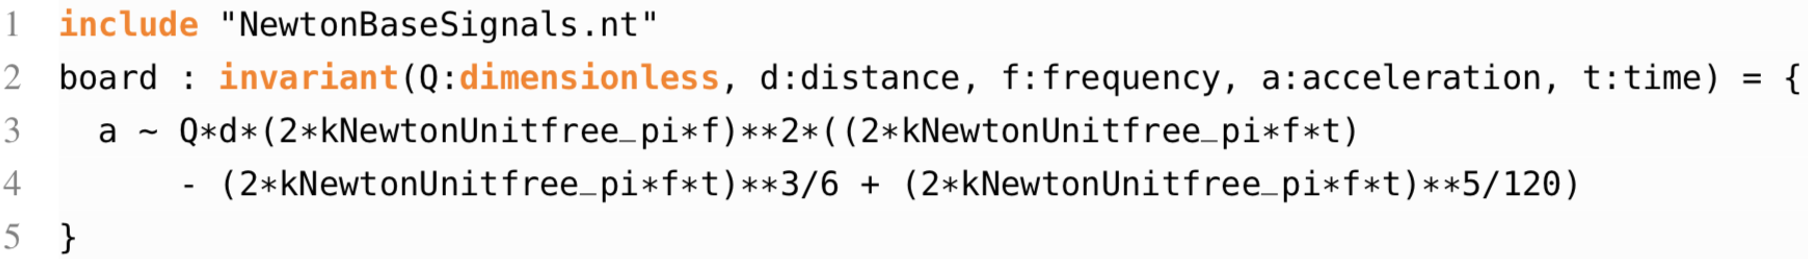
\includegraphics[width=\textwidth]{fig/newton_description.png}
      \caption{Example of a Newton description for a physically resonating circuit board (modelled in two dimensions) governed by Equation \ref{eqn:board_resonance}. Figure sourced from a poster produced in parallel to this project~\cite{eurosys_poster}.}
      \label{fig:newton_description}
    \end{figure}

    \begin{equation}
      a = Q_{bd} d_{bd} \omega^2sin(\omega t),
      \label{eqn:board_resonance}
    \end{equation}

    where:
    \begin{itemize}
      \item $a$ represents board acceleration,
      \item $Q_{bd}$ represents quality factor,
      \item $d_{bd}$ represents board displacement amplitude,
      \item $\omega$ represents angular resonant frequency,
      \item $t$ represents time.
    \end{itemize}

    \begin{figure}[H]
      \centering
      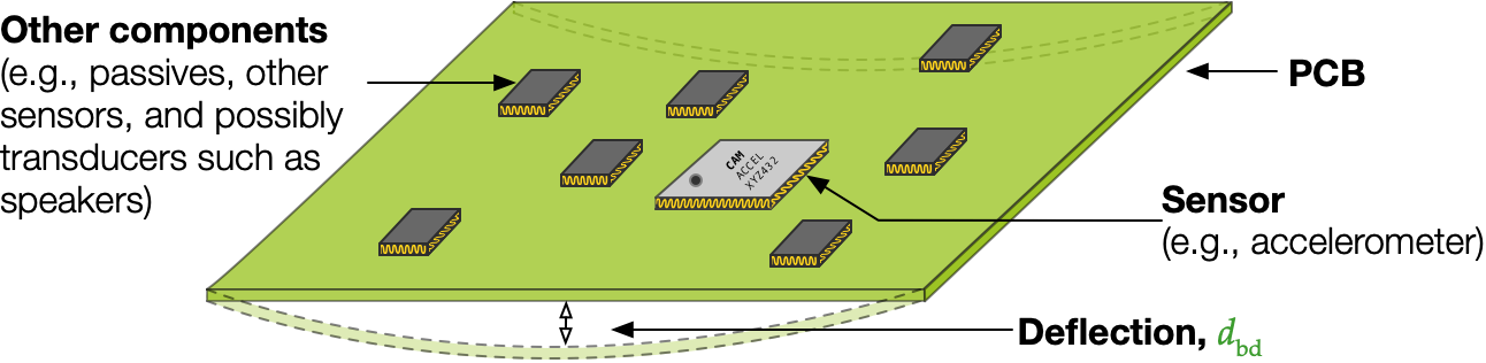
\includegraphics[width=0.75\textwidth]{fig/resonating_board.png}
      \caption{The system modelled by Equation \ref{eqn:board_resonance}. Figure sourced from a poster produced in parallel to this project~\cite{eurosys_poster}.}
      \label{fig:resonating_board}
    \end{figure}

    At the time of writing the Newton language and compiler is still under development by the Physical Computation Laboratory~\cite{physcomp}; the Newton compiler frontend is able to transform a human-readable Newton description into an intermediate representation, a tree structure that can be easily traversed by a computer. The motivation for this project was the idea that this information could be used by a compiler backend to generate a hardware description (e.g. Verilog). Within the context of this project, Newton provides the ability to describe the relationships between the sensors in a multi-sensor embedded system. This information is necessary to be able to quantify privacy losses in a multi-sensor system.

  \subsection{Random Number Generation} \label{subsection:intro_rng}
    One important component of a local differential privacy system is a true random number generator (TRNG) to generate the random noise used to obscure \textit{private} data\footnote{In a security related application, pseudorandom number generators such as linear feedback shift registers are unsuitable since an attacker would be able to predict their output}. The Laplace mechanism requires random noise to be Laplace distributed, introducing additional complexity compared to uniform or Gaussian distributed RNGs. The resource constraints imposed by the iCE40 FPGA dictated the need to implement a hardware efficient RNG to generate this Laplace distributed noise. A research article by De Schryver et al.~\cite{DeSchryver} outlines a possible architecture for such a system, based on a lookup table indexed by a floating point representation of the output of a uniform random number generator. This architecture was implemented in Verilog and analysed as part of this project (see Section \ref{subsection:rng_impl}).
\newpage



%
% THEORETICAL DEVELOPMENT
%

\section{Theoretical Development}
  The early stages of the project involved brainstorming and investigating potential research problems that would involve compiling Newton descriptions into a hardware description language. It soon became apparent that the Newton language was well suited to describing the relationships between sensors in a multi-sensor embedded system, thereby providing a basis to build upon the single-sensor state-of-the-art~\cite{Choi2018GuaranteeingLD}~\cite{diffpriv_2006}.
  \subsection{Brainstorming Example Applications}
    Below are some examples of security/privacy related applications of compiling a Newton description into Verilog that eventually led to the project's focus on differential privacy for multi-sensor systems.
    \subsubsection{Digital Camera/Viola-Jones Facial Detection}
      iCE40 FPGAs are able to drive digital cameras and perform facial recognition, as illustrated by the iCE40 Ultraplus Mobile Development Platform~\cite{iCE40_MDP}. In this context a differential privacy system might aim to apply random noise to an image in such a way that the identity of an individual can be obscured whilst still preserving enough information for facial detection algorithms to function correctly.  A Python script available in this report's GitHub repository\footnote{See Section \ref{subsection:GitHub}.} demonstrates this idea using OpenCV~\cite{opencv-contrib-python} --- the script converts a photo of a face to greyscale and subsamples to 32x32 size (effectively low pass filtering to remove high spatial frequencies) before Laplace distributed random noise ($\lambda$ = 25, mean = 0) is added to the pixel intensity values, similarly to the Laplace method described in Section \ref{intro_diff_priv}. The script then uses a Viola-Jones~\cite{Viola01rapidobject} classifier to detect faces in the images before and after the application of noise, demonstrating that a face can be detected in both cases provided the variance of the noise distribution is not too great to drown out all relevant information (analogous to the $\epsilon$ value in Section \ref{intro_diff_priv} being too small).\\

      The results of running this script can be observed in Figure \ref{fig:viola_jones}; the addition of random noise somewhat obscures the identity of the subject in the photo whilst still allowing a Viola-Jones facial detection to function. The demonstration featured here is a simple proof-of-concept; random distortion could be applied to the image in many different ways e.g. random displacement of pixels.

      \begin{figure}[H]
        \centering
        \subfloat[Original photo]{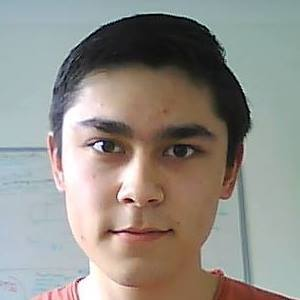
\includegraphics[width=0.3\textwidth]{fig/face.jpg}}
        \subfloat[Subsampled greyscale image]{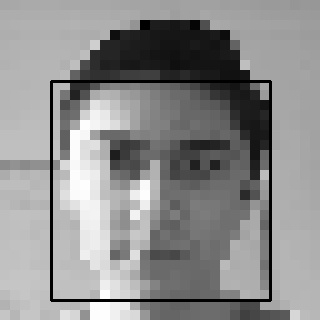
\includegraphics[width=0.3\textwidth]{fig/resized_image.jpg}}
        \subfloat[Random noise added]{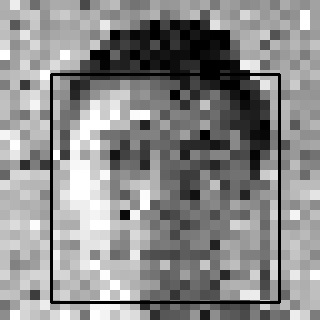
\includegraphics[width=0.3\textwidth]{fig/noised_image.jpg}}
        \caption{Proof-of-concept demonstration of Laplace distributed random noise being used to obscure an individual's identity whilst preserving a detectable facial structure. A square has been drawn around the faces detected by the pre-trained Viola-Jones classifier bundled with OpenCV. The photo features, and was taken by the author.}
        \label{fig:viola_jones}
      \end{figure}

      The Viola-Jones classifier works by applying rectangular filters to detect facial features. A Newton description could contain invariants to describe these filters in terms of pixel values; this information could, for example, be used by a noising system to ensure that random noise is applied in a way that does not significantly impact an image's response to the facial detection filters (i.e. if an image contains a face, then the Viola-Jones classifier described in Newton should still detect the face after the noising process, and vice versa if no face is present in the un-noised \textit{private} image).

    \subsubsection{Microphone}
      In a similar manner to the camera example above, noise could be added to audio data in such a way that a person's voice can be masked whilst still preserving features, such as mel-frequency cepstral coefficients, that allow speech recognition algorithms to function. The Newton language would be used to describe invariants in the time and/or frequency domains that must be held during the noising process.

    \subsubsection{\textit{Intelligent} Noising}
      This project investigates a system which allows a user to specify which measurement signals they wish to add random noise to. It is possible to generalise this idea to a hypothetical system which has control over how it applies random noise to measurement data in order to mask a more abstract form of information. One concrete example of this would be when working with images (e.g. the  Viola-Jones example above) --- given the requirement that individuals' identities should be obscured whilst still providing enough information for facial detection algorithms to work reliably, a system might choose to apply noise using, for example:

      \begin{itemize}
        \item Random noise added to pixel intensities.
        \item Convolution with a random filter.
        \item Random rearrangement of pixels.
        \item A combination of multiple techniques.
      \end{itemize}

      For such a system, a Newton description could be used to define constraints on the noised image's response to the Haar-like features used by a particular Viola-Jones facial detection algorithm; the system would then randomise the image in such a way that the constraints are not violated i.e. both the unnoised and noised images exhibit similar features, producing similar results when the face detection algorithm is applied.

\section{System Design and Implementation}
  \subsection{Privacy Budget Management System Architecture} \label{subsection:privacy_budget_system_arch}
    The following section proposes a privacy management system architecture that could be used to manage multi-sensor privacy on an FPGA. Due to project time constraints, the system has not been completely implemented, since this would divert time and attention away from investigating the more important research questions posed by the project. The progress made so far by the author is documented in sections \ref{section:tech} and \ref{section:characterisation}.
    \\

    \textit{$\langle$ TODO: describe what will have been implemented by the submission date e.g. use privacy yaml file and Newton AST to generate some of the logic implementation by filling in a Verilog template$\rangle$}
    \\
    
    The proposed system architecture is as follows:
    \begin{itemize}
      \item The FPGA acts as a sensor interface, allowing external circuitry to request noised sensor values. Noised measurement signals are referred to as \textit{protected}, as their true value has been masked by the addition of zero-mean Laplace distributed random noise to preseve privacy; the system also allows \textit{unprotected} signals to be forwarded to the outside world with no random noise added. %Newton also allows signals to be derived from other more fundamental signals e.g. a value derived from sensor measurements; for this system, random noise can only be applied to sensor measurement signals i.e. these are the only types of signal that can be (and the only types of signal that need to be) protected.
      \item A \textit{privacy file} (e.g. a YAML file) is used to specify protected measurement signals for a particular embedded system.
      \item In order to apply random noise to a particular signal, a range of parameters must be defined for each protected signal:
      \begin{itemize}
        \item Range of possible sensor outputs.
        \item \textit{Privacy budget} value allocated to the sensor.
        \item \textit{Privacy budget} replenishment rate.
        \item Value of $\epsilon$, a measure of privacy where a smaller value results in greater privacy by increasing the variance of applied noise~\cite{Choi2018GuaranteeingLD}.
      \end{itemize}
      These values can be provided for each protected signal within the \textit{privacy file}.
      \item The FPGA maintains a differential privacy \textit{budget} for each protected signal. Querying a value for a protected signal (i.e. requesting a noised measurement from the FPGA) causes that signal to incur a privacy loss. The FPGA quantifies this loss (a function of the random noise sample added to the raw measurement~\cite{Choi2018GuaranteeingLD}) and subtracts it from the signal's privacy budget. Once the budget is depleted, further queries of the signal in question are ignored --- a nonzero budget replenishment rate can be specified in the privacy file so that the signal can eventually be queried again once the budget has replenished sufficiently.
      \item Invariants in the Newton description define relationships between signals. This is important as privacy is lost if a measurand's value is calculated by taking measurements from related sensors, without directly measuring the measurand. The system must account for this \textit{indirect} privacy loss:
      \begin{itemize}
        \item Each Newton invariant containing protected measurement signals has an associated bitfield register on the FPGA. Each bit in the register acts as a read flag for each measurement signal contained in the associated invariant --- the flag is set when the sensor is queried (i.e. when a measurement is taken and the noised measurement value becomes \textit{known} to the outside world) and is not cleared until the sensor's privacy budget is completely replenished some time after a query (at which point the measurement value can be considered \textit{unknown} to the outside world).
        \item As long as any two flags remain unset, there are two variables in the equation that are \textit{unknown} to an attacker. The equation cannot be solved and so no information\footnote{This assumes that the probability distributions of sensor outputs are independent, see Appendix \ref{appendix:diff_priv_loss} for an investigation into correlated measurements.} can be gained about the \textit{unknown} values.
        \item If only one bit remains unset, then the remaining \textit{unknown} value can be calculated using the other \textit{known} values with set flags --- the \textit{unknown} signal incurs a privacy loss. If all flag bits are set then responding to a measurement query results in a privacy loss for every other signal in the invariant. These scenarios can be summarised by saying that, for signals contained within a particular Newton invariant, a signal experiences an indirect privacy loss if any of the other signals in the invariant are queried \textit{and} all other signals are \textit{known} i.e. have been recently queried.
        \item If responding to a query would exceed the privacy budget for any protected signal (not just the one being queried) then a response should not be granted.
      \end{itemize}
      \item The mathematics behind the calculation of a quantitative value for privacy loss is investigated in Appendix \ref{appendix:diff_priv_loss}; whilst calculation of an exact value for privacy loss (Equation \ref{eqn:exact_indirect_priv_loss} in Appendix \ref{appendix:diff_priv_loss}) requires the use of a mathematical optimisation technique such as Lagrange multipliers, a simpler calculation can be used to obtain an upper bound on the value. This simpler calculation can be performed more easily on a small FPGA such as the iCE40, and can even be pre-calculated during compile-time since it is a function of the random noise output only.

    \end{itemize}

    \subsection{FPGA}
      This system is based on the iCE40 UP5K FPGA~\cite{iCE40}, selected for its small size and low power consumption. These qualities make it ideal for inserting into an embedded device without significantly impacting the size or power consumption/battery life. Using FPGA hardware rather than a software implementation running on a processor has several advantages:

      \begin{itemize}
        \item Increased speed, to the point where data rate is limited by the SPI/I2C bus clock rather than the privacy system.
        \item Increased energy efficiency.
        \item Potential for integration into a sensor's package (due to the FPGAs small size).
        \item Security - a hardware implementation is difficult for an attacker to manipulate or modify.
      \end{itemize}

    \subsection{Hardware Entropy Source} \label{subsection:hardware_entropy_source}
      As discussed in section \ref{subsection:intro_rng}, one of the key components of a security/privacy application is a true random number generator (TRNG). Unlike a pseudorandom number generator (PRNG), which produces a predictable deterministic outcome, a true random number generator's output cannot be anticipated by an attacker, preserving system security and users' privacy. The output bit rate of TRNGs is often limited so can be used to seed a cryptographically secure PRNG (CSPRNG) algorithm to increase output bit rate without significantly compromising security. This extra step was not required for this project, since the rate at which random numbers are consumed is relatively low.\\

      Initial investigations focused on using the iCE40 FPGA's differential I/O hardware to generate random bits which could be fed into a TRNG to generate random samples from an arbitrary distribution. Initially, it was hoped that simply leaving two comparator inputs floating would cause the output to fluctuate randomly --- in practice this did not occur as the comparator hardware requires one of the inputs to be biased within a narrow common mode voltage range (roughly half the I/O supply voltage, allowing the other input to swing about this reference voltage)~\cite{ice40_diff_io}. The author decided to design a PCB to set this bias voltage, as well as provide an alternative entropy source in the form of a reverse biased avalanche diode producing avalanche noise. In theory, this circuit would provide a better i.e. less predictable source of entropy since, unlike the floating input pin, the avalanche noise (and therefore random number output) produced is independent of the device's external environment\footnote{A floating input pin can easily be influenced by its external environment e.g. picking up 50Hz noise from nearby electrical mains, resulting in a non-uniform frequency spectrum for random output.}.\\

      The circuit used in this noise generator is based on a design by Professor Paul Horowitz~\cite[p.~984]{art_of_electronics}, modified to operate at 3.3V and 0V power rails (rather than $\pm5V$). Avalanche noise produced by a reverse biased base-emitter junction of a 2N4401 transistor is amplified through a dual op-amp amplifier stage before being modulated about a 1.65V DC bias $\left(\frac{V_{cc}}{2}\right)$; this output can then be fed into one of the iCE40's comparator inputs. A second output on the PCB comes from a simple potentiometer circuit to set the common mode reference voltage on the second comparator input (with series resistors to allow for fine control about $\frac{V_{cc}}{2}$). Since the comparator output depends on whether the instantaneous voltage of the noise waveform lies above or below this reference voltage, this reference point can be adjusted to set the ratio of ones to zeros in the random comparator output.\\

      The Art of Electronics~\cite[p.~984]{art_of_electronics} describes the avalanche noise produced by the circuit as being spectrally white up to around 50MHz, whilst the output signal has a 100mV RMS voltage.

      \begin{figure}[H]
        \centering
        \subfloat[Front]{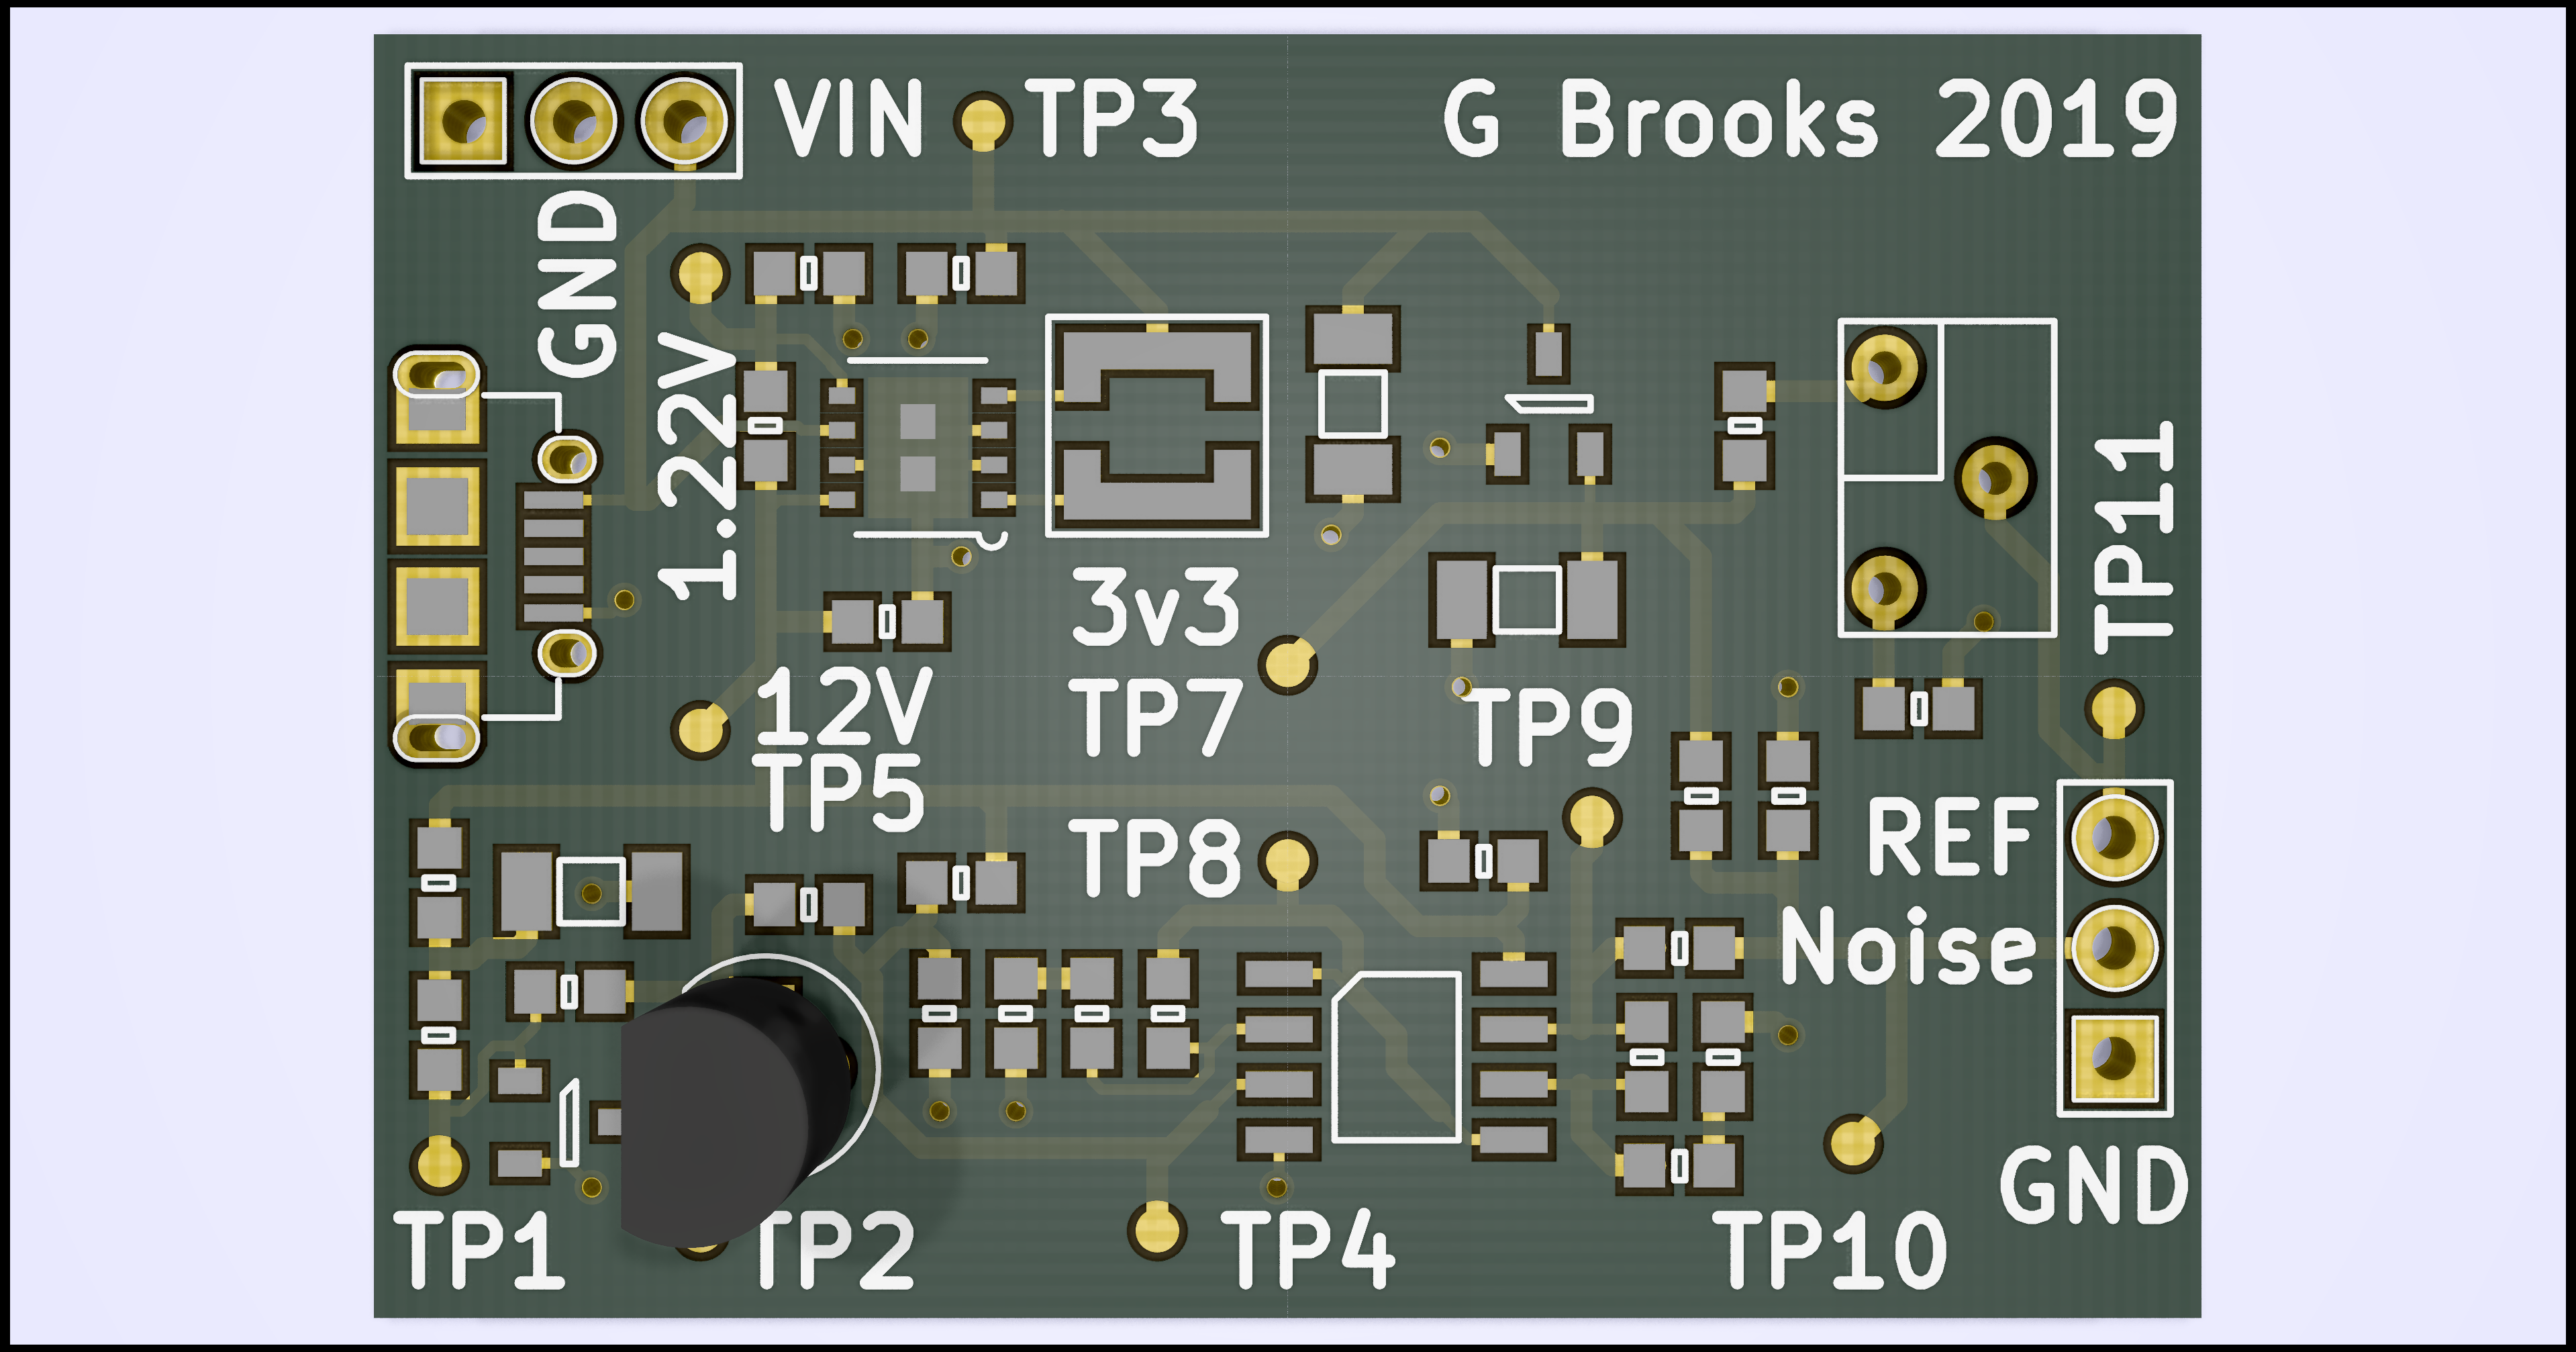
\includegraphics[width=0.4\textwidth]{fig/pcb_render_f.png}}
        \subfloat[Back]{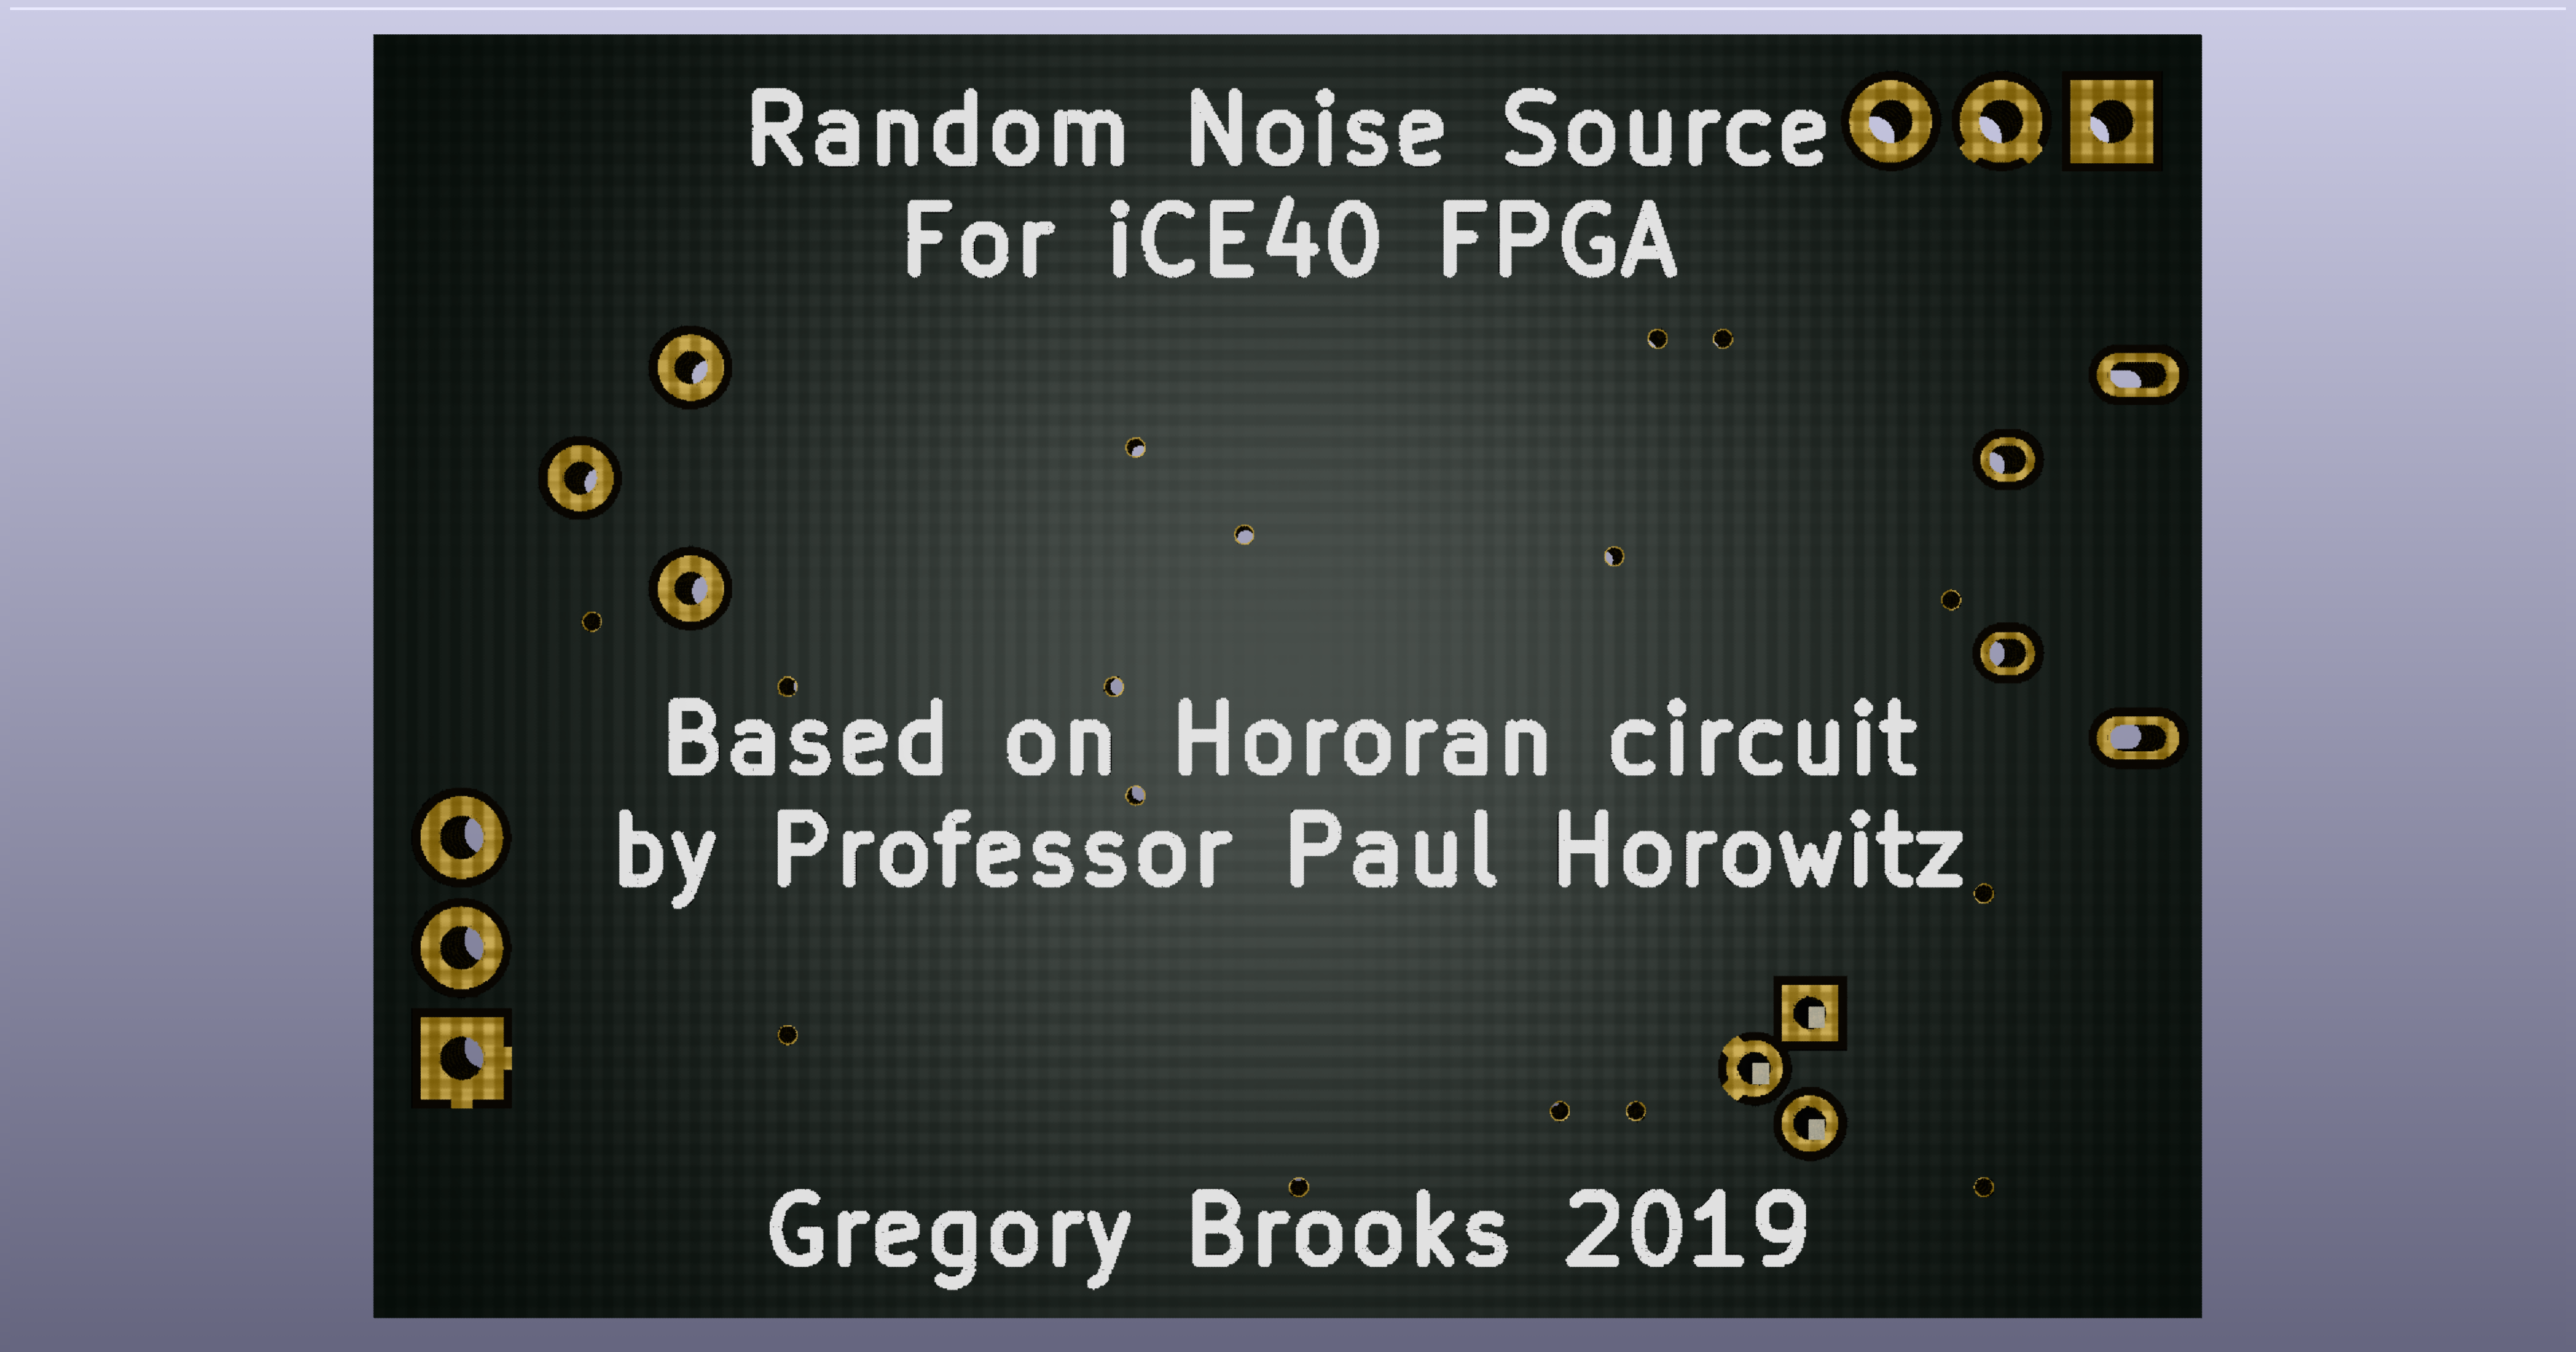
\includegraphics[width=0.4\textwidth]{fig/pcb_render_b.png}}
        \caption{3D renders of PCB (in KiCad).}
        \label{fig:pcb_render}
      \end{figure}

      The full circuit schematic and PCB layout can be found in Appendix \ref{appendix:schematic}, as well as the GitHub repository listed in Section \ref{subsection:GitHub}.

      \subsection{Uniform Random Number Generator} \label{subsection:urng_impl}
        \begin{figure}[H]
          \centering
          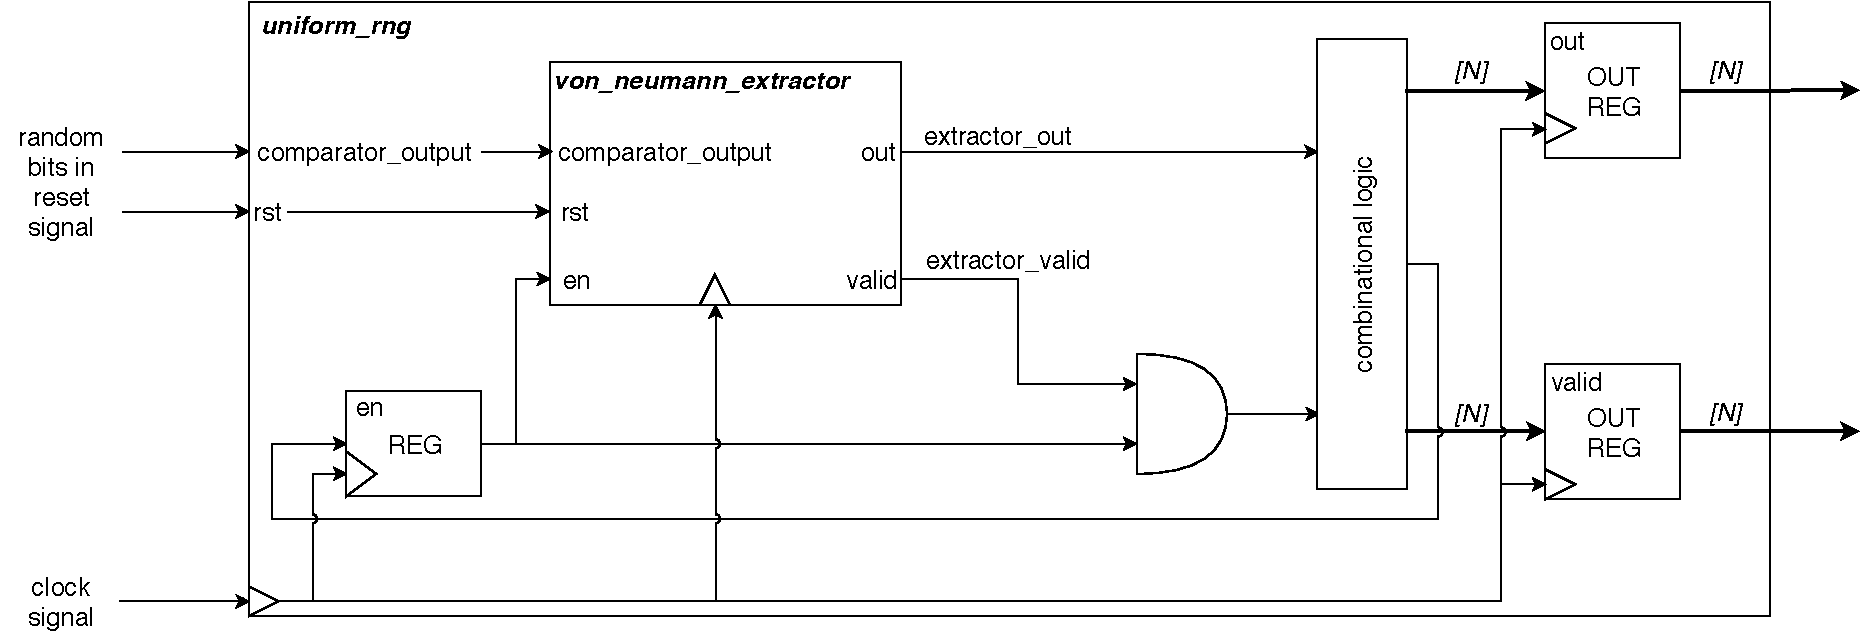
\includegraphics[width=\textwidth]{fig/urng.pdf}
          \caption{Block diagram of URNG logic circuit.}
          \label{fig:urng_block_diagram}
        \end{figure}

        Figure \ref{fig:urng_block_diagram} shows the logic circuit for the uniform random number generator described in Verilog as part of this project (see Section \ref{subsection:GitHub} for the GitHub repository containing the code). Random bits are supplied to this logic circuit, such as those produced by the hardware entropy source described in Section \ref{subsection:hardware_entropy_source}. These are fed into a von Neumann debiasing module that uses a simple algorithm, invented by John von Neumann, to remove bias from the input bits, so that the probability of reciving a 1 bit from the debiasing module's output is equal to the probability of receiving a 0. This is achieved by taking two input bits at a time --- if both bits are equal (received sequence 0,0 or 1,1), they are discarded; if the received sequence is 1,0 then the output bit is 1; if the received sequence is 0,1 then the output bit is zero. The module's behaviour can be described more formally: for random input bits modelled by random variable $X$ with a distribution $p()$ such that $p(X = 1) \neq p(X = 0)$ but $p(X_i = 1, X_{i+1} = 0) = p(X_i = 0,X_{i+1} = 1)$, the debiasing module outputs random bits modelled by random variable $Y$ with distribution $q()$ where $q(Y=0) = q(Y=1)$.\\

        The additional logic in this URNG module is used to store $n$ bits output by the extractor in an $n$ bit output register (providing a fixed point $n$ bit uniform random number). Each bit in the register is associated with a valid signal (stored in the \textit{valid} output register) that goes high once the associated output bit takes on a value from the extractor output.\\

        The circuit runs until the output register is filled, at which point the internal enable (\textit{en}) register is set from 1 to 0; to generate a new random number the module must be reset.\\

        The GitHub repository for the URNG contains a Verilog testbench that can be run with the command \texttt{make simurng} to successfully simulate and test this logic circuit. The circuit has also been successfully synthesised for an iCE40 UP5K FPGA; a detailed analysis is presented in Section \ref{subsection:scaling}.

      \subsection{Inversion Method Random Number Generator} \label{subsection:rng_impl}
        \begin{figure}[H]
          \centering
          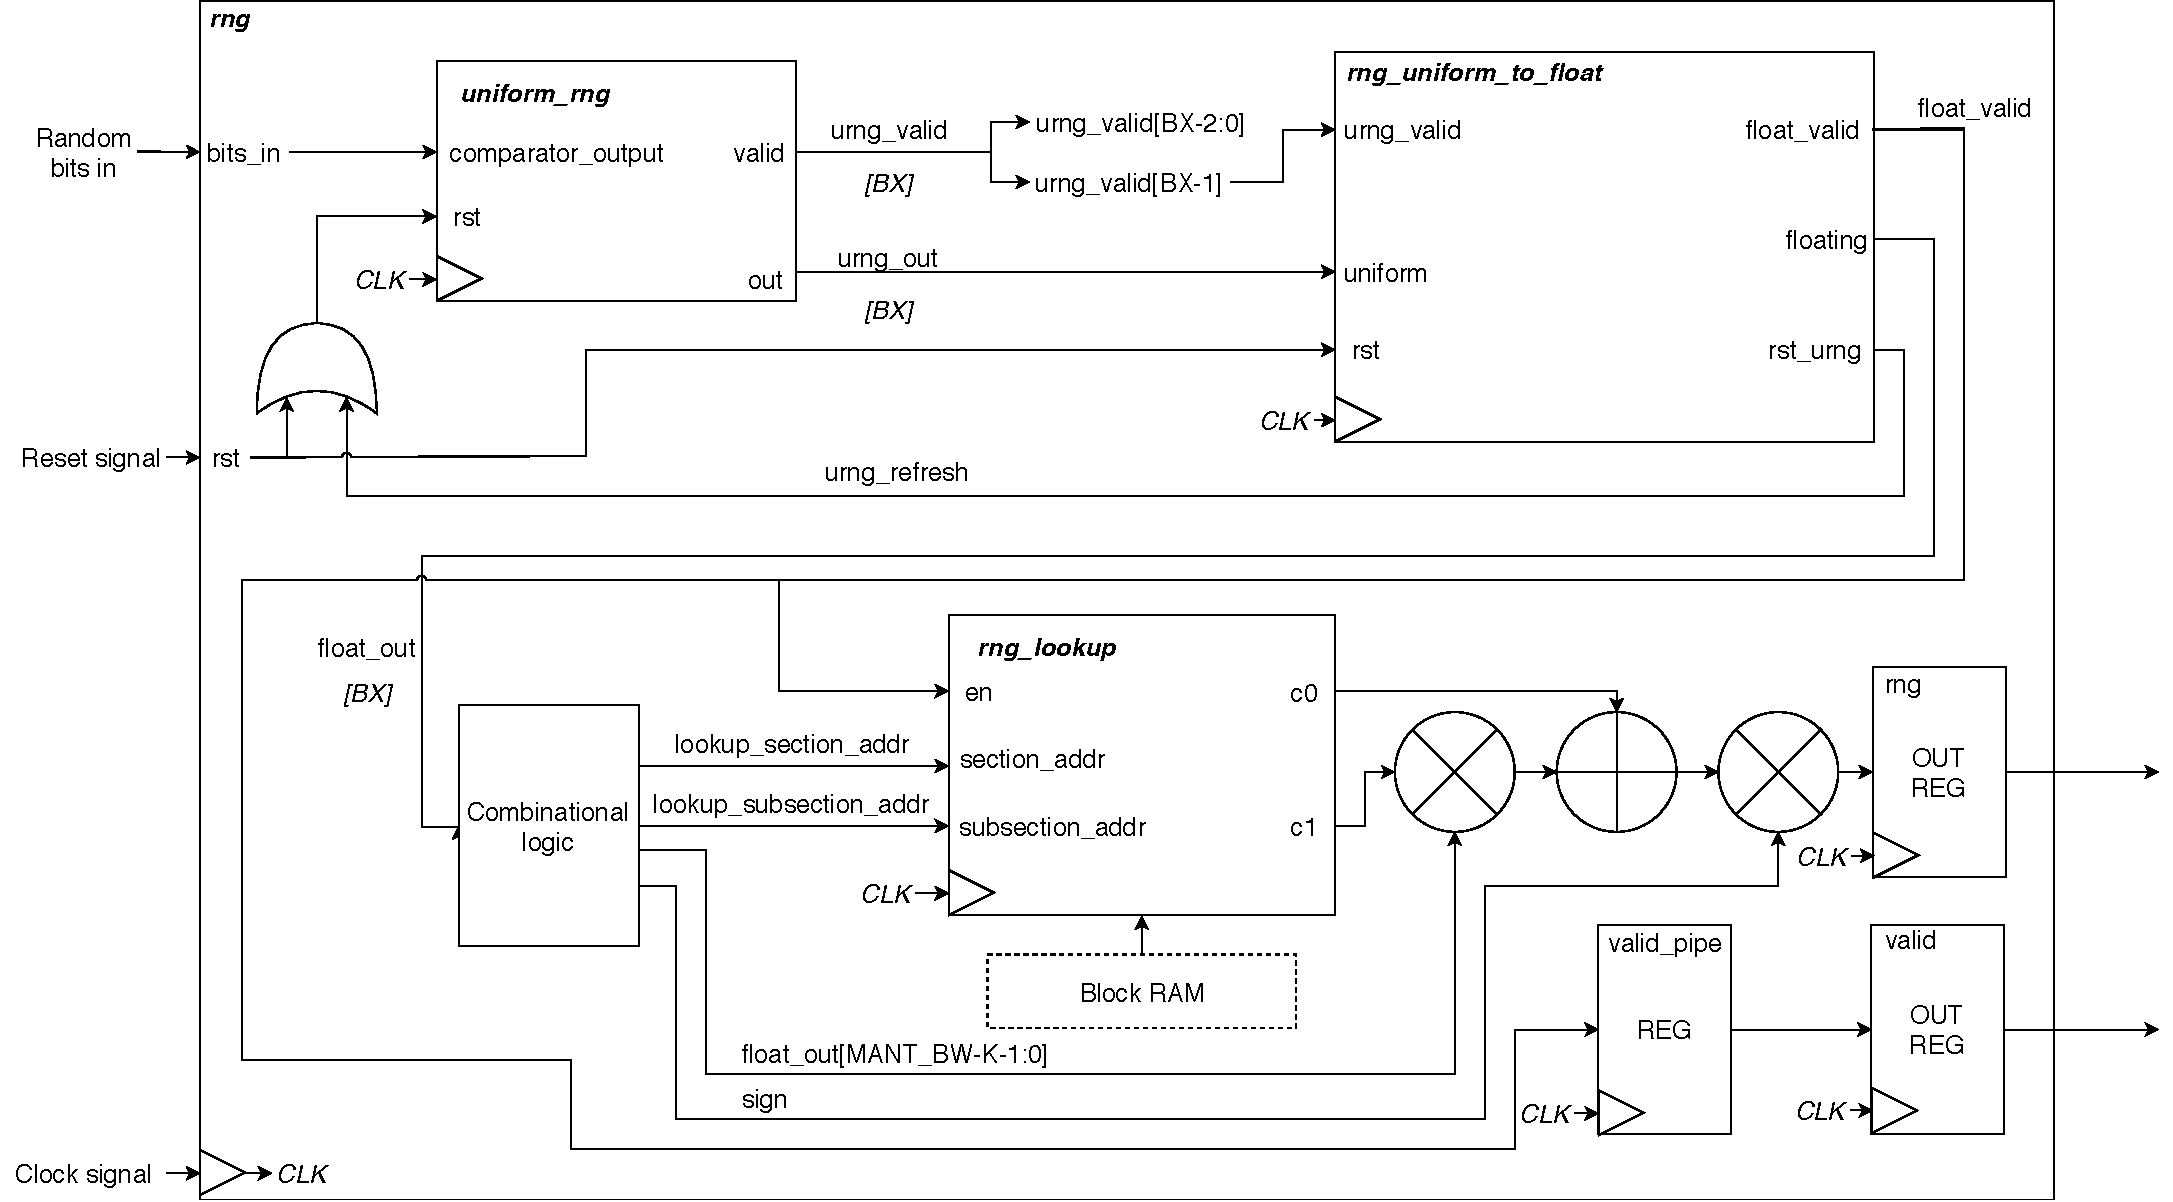
\includegraphics[width=\textwidth]{fig/rng.pdf}
          \caption{Block diagram of RNG logic circuit.}
          \label{fig:rng_block_diagram}
        \end{figure}

        This module contains the URNG described in Section \ref{subsection:urng_impl}, transforming uniformly distributed random numbers into random numbers distributed according to an arbitary (e.g. Laplace) distribution. This is achieved by implementing the hardware efficient system described by De Schryver et al.~\cite{DeSchryver}.\\

        The module \textit{rng\_uniform\_to\_float} takes the uniform random numbers produced by the URNG and transforms them into a floating point representation using the algorithm described by De Schryver et al.~\cite{DeSchryver}. The production of a single floating point number may require more than one uniform random number to be consumed, so this module is capable of resetting the URNG to generate as many uniform random numbers as it needs to produce a floating point output number. This module requires an internal block of combinational logic to count the number of leading zeros within a particular region of the bit vector coming from the URNG; the author implemented this logic module using a hardware-efficient recursively\footnote{The finite recursion depth when instantiating this module means that the resulting logic circuit is still synthesisable i.e. can be realised as a physical circuit on an FPGA.} instantiated tree structure proposed by Oklobdzija~\cite{clz}.\\

        The floating point number produced by the \textit{rng\_uniform\_to\_float} module is used as the input address to a block RAM lookup table, allowing two coeffients (c0 and c1) to be read out of the RAM. The contents of this RAM is generated by a C program written by the author (described in Section \ref{subsection:build_system}) which obtains c0 and c1 coefficients by taking discrete samples of a continuous probability distribution such as the Laplace distribution. The final output number is calculated at $c0 + c1 \times m$ where $m$ consists of a certain number\footnote{Details of this random number generator architecture can be found in the paper~\cite{DeSchryver} on which this implementation is based; they are not repeated in this report.} of the least significant bits from the mantissa part of the floating point number produced by \textit{rng\_uniform\_to\_float}. This final random number output is accompanied by a valid flag signal; this signal must be delayed using the \textit{valid\_pipe} register to synchronise it with the associated random number at the output. As with the URNG, the logic circuit runs until a valid random number appears at the output; it must then be reset to produce a new random number.

\newpage



%
% TECHNOLOGIES AND TECHNIQUES USED
%

\section{Technologies and Techniques Used} \label{section:tech}
  \subsection{Git/GitHub} \label{subsection:GitHub}
    Below is a list of GitHub repositories containing work done as part of this project:
    \begin{itemize}
        \item Main project repository containing Python simulations/tests, Verilog templates, Verilog hardware descriptions (e.g. the nonuniform random number generator) and C code:\\
        \url{https://github.com/Gregox273/Newton-Verilog-Compiler}
        \item Verilog repository for the iCE40 differential I/O based uniform random number generator:\\
        \url{https://github.com/physical-computation/iCE40-LVDS-RNG}
        \item Schematic and PCB design for hardware random noise generator:\\
        \url{https://github.com/Gregox273/hardware-rng}
        \item Physical Computation Laboratory measurement repository, containing measurements taken when characterising the hardware random number generator (Sections \ref{subsection:eval_hardware_entropy} and \ref{subsection:eval_randomness}):\\
        \url{https://github.com/physical-computation/measurement-data}\\
        Measurement Number: 33
        Branch: issue-33

    \end{itemize}

    Over the course of this project, GitHub provided a remote location to store/backup work and transfer it between computers. Git's version control functionality facilitated development of software, Verilog firmware and documentation by allowing work to be divided up into commits that could be merged/rolled back/compared when necessary. The Git commit history also provides a timeline of project progress --- an example is shown in Figure \ref{fig:commits}.

    \begin{figure}[H]
      \centering
      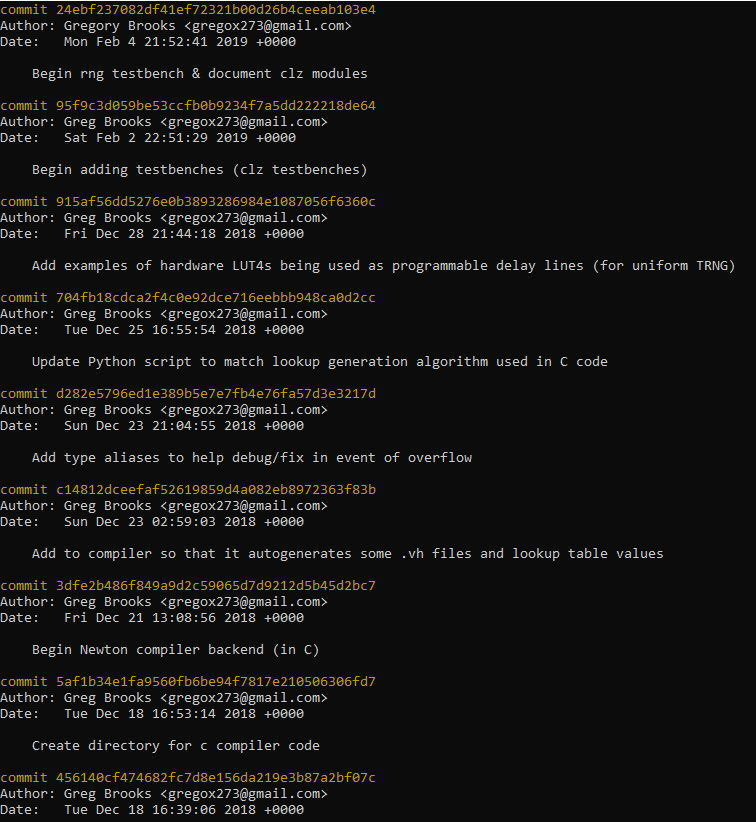
\includegraphics[width=\textwidth]{fig/commits.png}
      \caption{Example of the commit history for the main project repository (Newton-Verilog-Compiler).}
      \label{fig:commits}
    \end{figure}
    \clearpage

  \subsection{FPGA Synthesis Toolchain}
    The author used the open source Project IceStorm~\cite{icestorm} toolchain to synthesise Verilog code and to program the iCE40 FPGA. The following tools in the toolchain were used over the course of the project:
    \begin{itemize}
      \item Yosys: synthesises Verilog to a logic circuit representation.
      \item Arachne-pnr: place and route tool that maps a logic circuit to physical hardware within the FPGA.
      \item Icepack: tool for converting ASCII format file (e.g. the arachne-pnr output) to a binary file (bitstream) for programming the iCE40 FPGA.
      \item Icetime: tool used to analyse signal timings in the circuit to be programmed. One of the useful parameters output by this tool is a value for the maximum clock speed a circuit can be expected to operate at.
      \item Iceprog: a program used to program an iCE40 FPGA over USB, using an FTDI based programmer present on the board to be programmed.
    \end{itemize}

  \subsection{Main Project Repository Structure and Build System} \label{subsection:build_system}
    This section describes the layout of the \textit{Newton-Verilog-Compiler} main project repository, as well as the method used to compile/synthesise code contained within. This repository contains a significant amount of the work carried out as part of this project, but not all of it (see Section \ref{subsection:GitHub}).\\

    At the start of the project, the author decided to use Python scripts to prototype algorithms that would later be implemented in C or Verilog. This was done to aid debugging and testing due to the ease with which a Python script can be paused, inspected and restarted during execution (though it could be argued that a debugger such as gdb allows compiled C programs to be manipulated in a similar way). This Python script can be found in the \texttt{python-diff-priv} directory within the main repository.

    All Verilog modules written over the course of this project are parameterised so that wire/register bit widths can be easily changed without having to rewrite any code. In this repository, parameter values are taken from \texttt{.vh} Verilog header files which can be supplied manually or generated using the C program in the \texttt{c\_compiler} directory --- this program takes the privacy file \texttt{privacy.yaml} (a partial implementation of the \textit{privacy file} described in Section \ref{subsection:privacy_budget_system_arch}) as an input and uses it to generate Verilog header files, by populating a template file. The program also generates the data to be stored in the FPGA's block RAM as part of the random number generator's BRAM lookup table; this data is stored in \texttt{.mem} files that are read in Verilog using the \texttt{\$readmemh} command.\\

    The \texttt{c\_compiler} directory also contains the Verilog code for the nonuniform random number generator.\\

    Throughout this project, the author made extensive use of the \texttt{make} tool for Linux, simplifying the compilation/synthesis process:
    \begin{itemize}
      \item The C program is compiled by running \texttt{make} in the \texttt{c\_compiler} directory. It can then be run with \texttt{build/c\_compiler}.
      \item Once the C program has been run to generate the necessary Verilog header files and \texttt{.mem} BRAM initialisation value, the Verilog code for the nonuniform random number generator can be synthesised by running \texttt{make synthrng} in the \texttt{c\_compiler/verilog} directory. Alternatively \texttt{make simrng} can be used to simulate it, running a  Verilog testbench. Similar commands (\texttt{make synthclz}/ \texttt{make simclz}) can be used to synthesise/test the leading zero counter logic in isolation.
    \end{itemize}

\newpage



%
% EVALUATION AND CHARACTERISATION
%

\section{Evaluation and Characterisation} \label{section:characterisation}

  \subsection{Evaluation of Hardware Entropy Source} \label{subsection:eval_hardware_entropy}
    \begin{figure}[H]
      \centering
      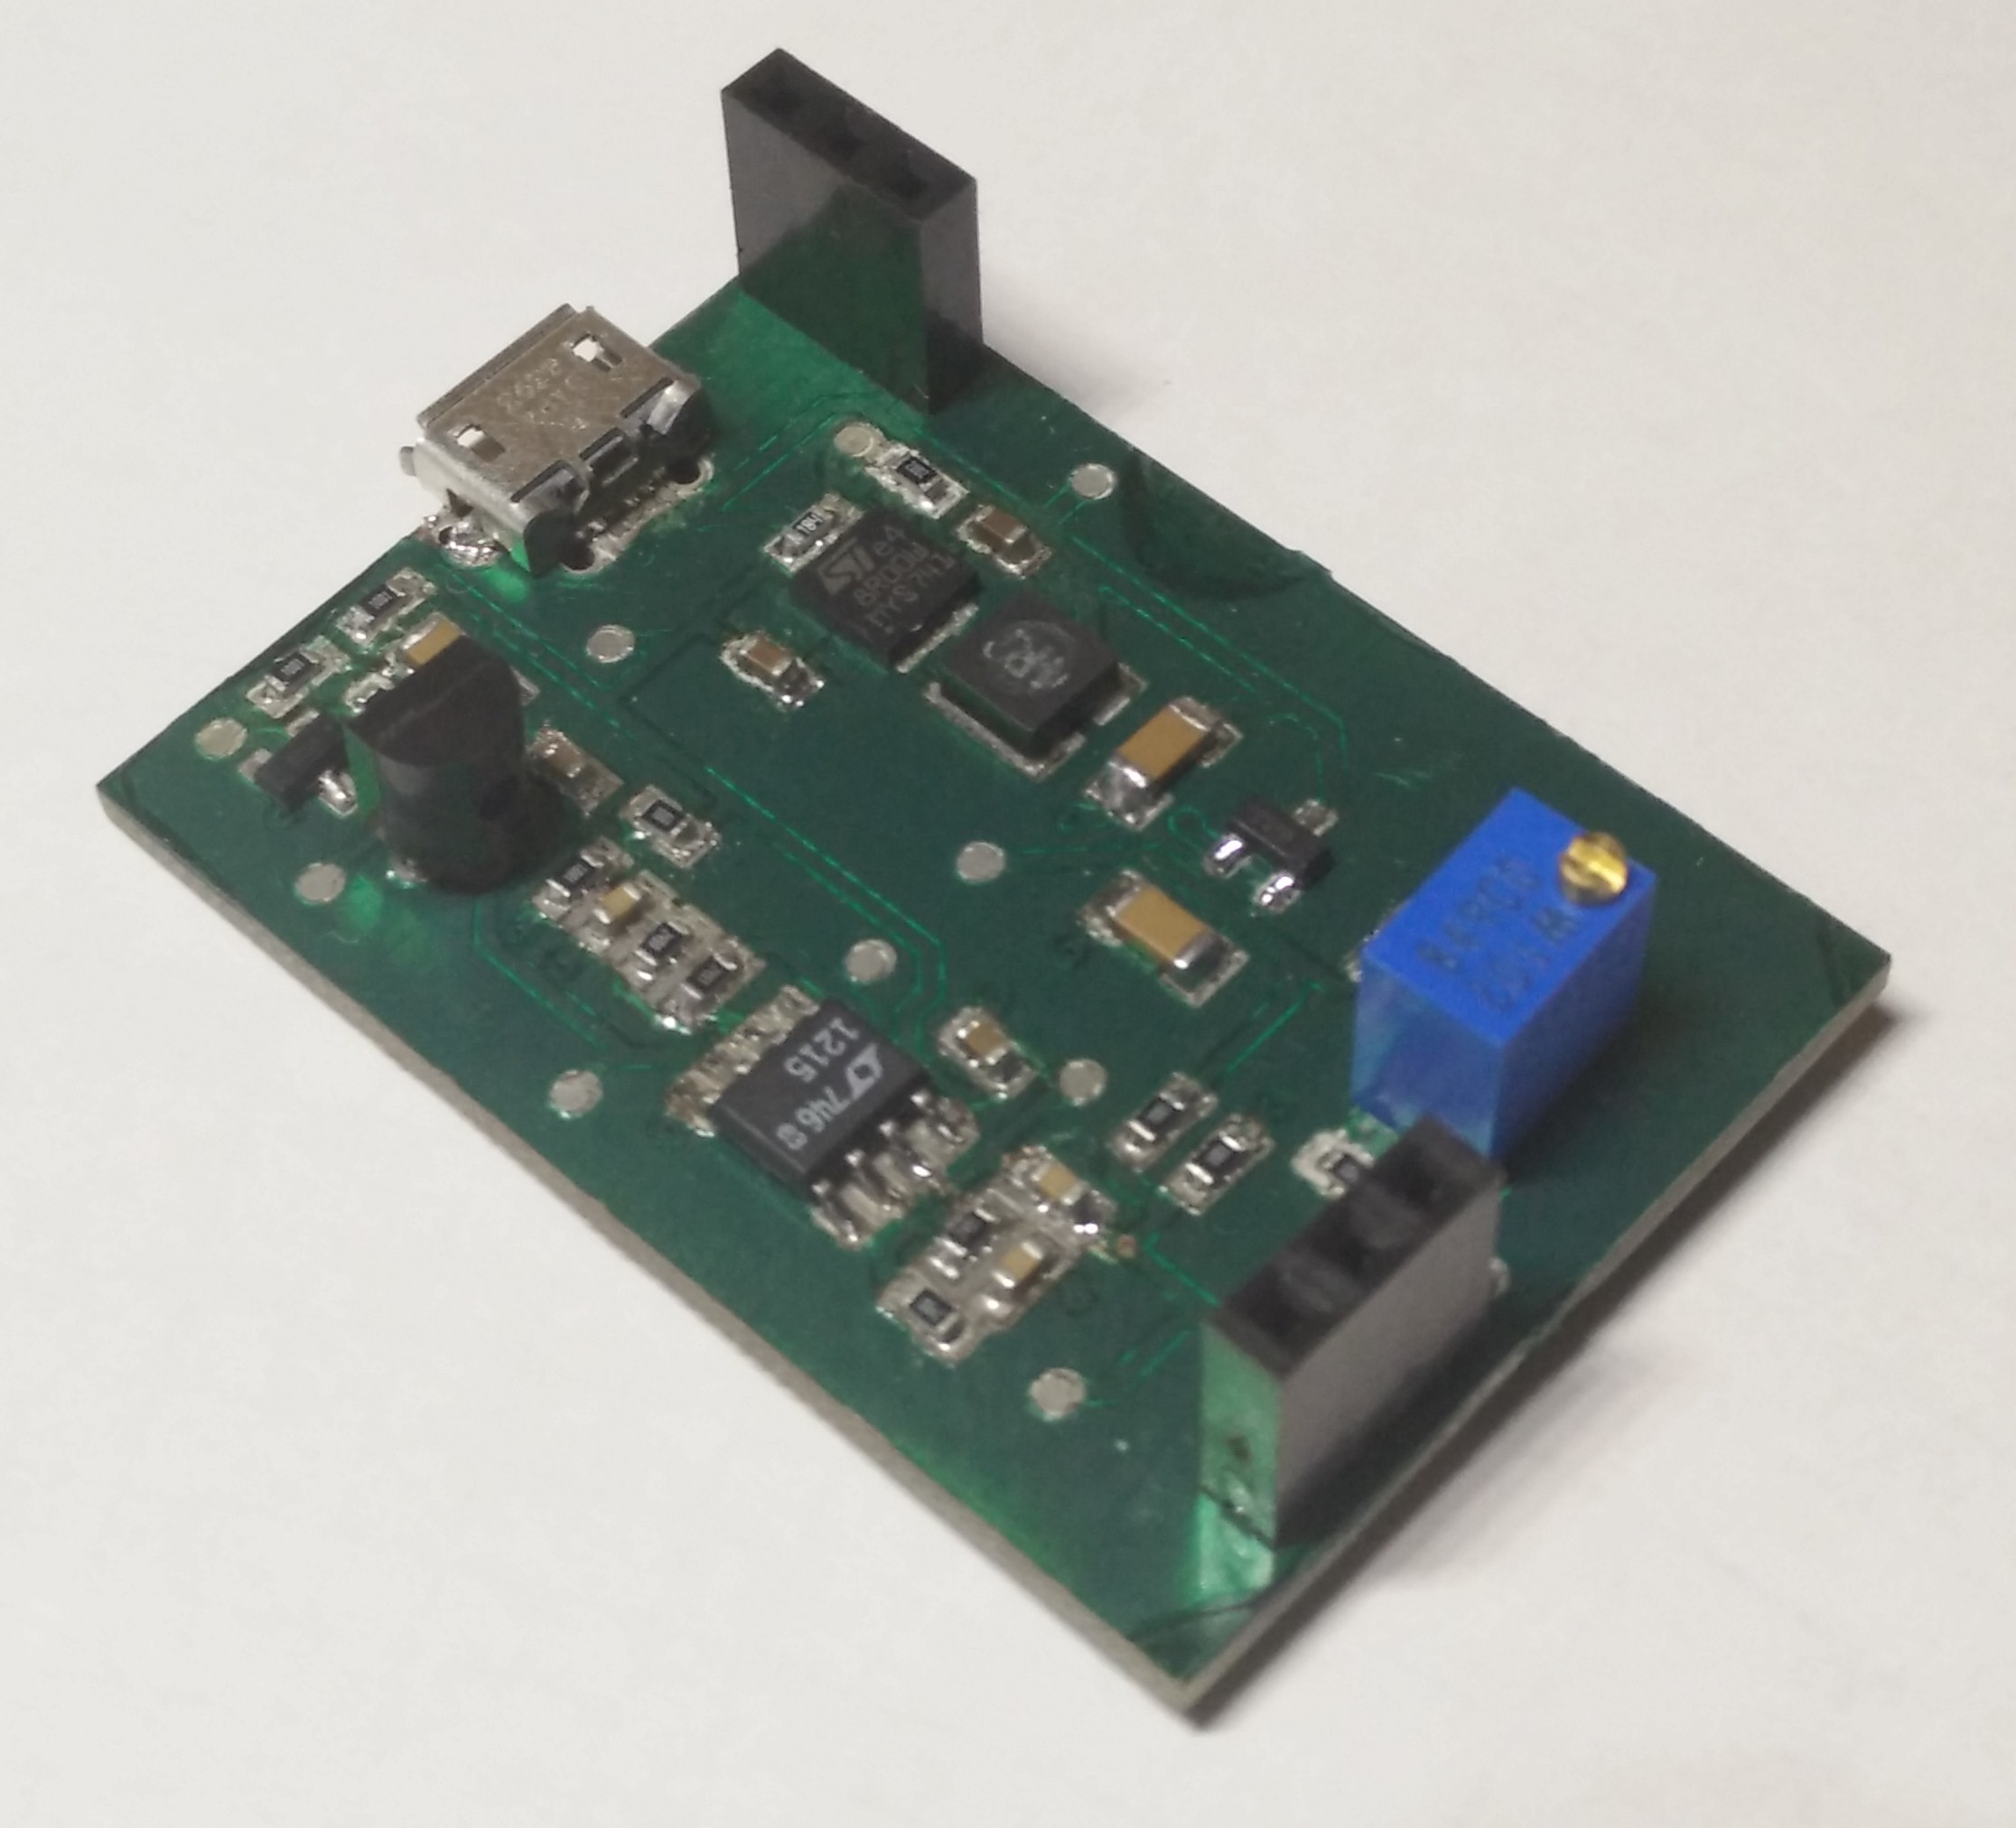
\includegraphics[width=0.5\textwidth]{fig/PCB_CROPPED.jpg}
      \caption{The physical PCB, assembled by the CUED Dyson Centre's Electronics Development Group.}
      \label{fig:pcb_cropped}
    \end{figure}

    \subsubsection{Method}
    This section presents measurements taken at several test points in the assembled circuit, analysing the noise signal at each stage in the amplifier circuit. A schematic is available in Appendix \ref{appendix:schematic}, showing the locations of these test points within the circuit. The author measured and recorded voltage waveforms at each of the testpoints listed below using a Tektronix MDO4104C oscilloscope with both AC and DC probe coupling --- DC coupling was used for the waveform screenshots shown below, (as well as for taking the average voltage measurements shown in the screenshots), whilst AC coupling was used for $V_{RMS}$ measurements. When displaying the FFT of signals on the oscilloscope, the author used a rectangular window function since the noise spectrum was predicted to be fairly wide (The Art of Electronics describes the avalanche noise as being white up to 50MHz~\cite[p.~984]{art_of_electronics}, whilst the op-amps used in this circuit have a gain-bandwidth product of 23MHz~\cite{lt1215}).

    \newpage
    \subsubsection{Results}

      % \newpage
      \paragraph{TP2: Avalanche breakdown noise source}

      % \begin{center}
      %   \begin{tabular}{ c c c }
      %      $V_{rms} = $ & , & $V_{av} = $
      %   \end{tabular}
      % \end{center}
      %
      % \begin{figure}[H]
      %   \centering
      %   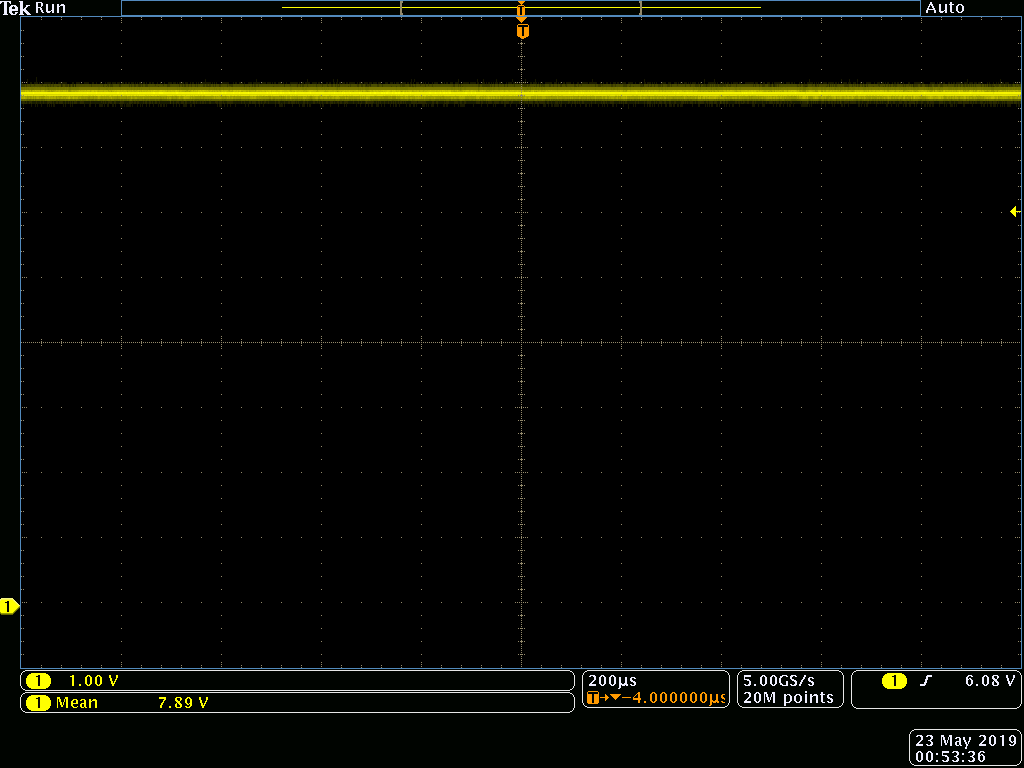
\includegraphics[width=0.5\textwidth]{fig/tp2_yt.png}% TODO: fill in
      %   \caption{Measured waveform with DC probe coupling. $V_{average} = $.}% TODO: fill in V_{average}
      %   \label{fig:tp2_waveform}% TODO: update label with appropriate TP number
      % \end{figure}
      %
      % \begin{figure}[H]
      %   \centering
      %   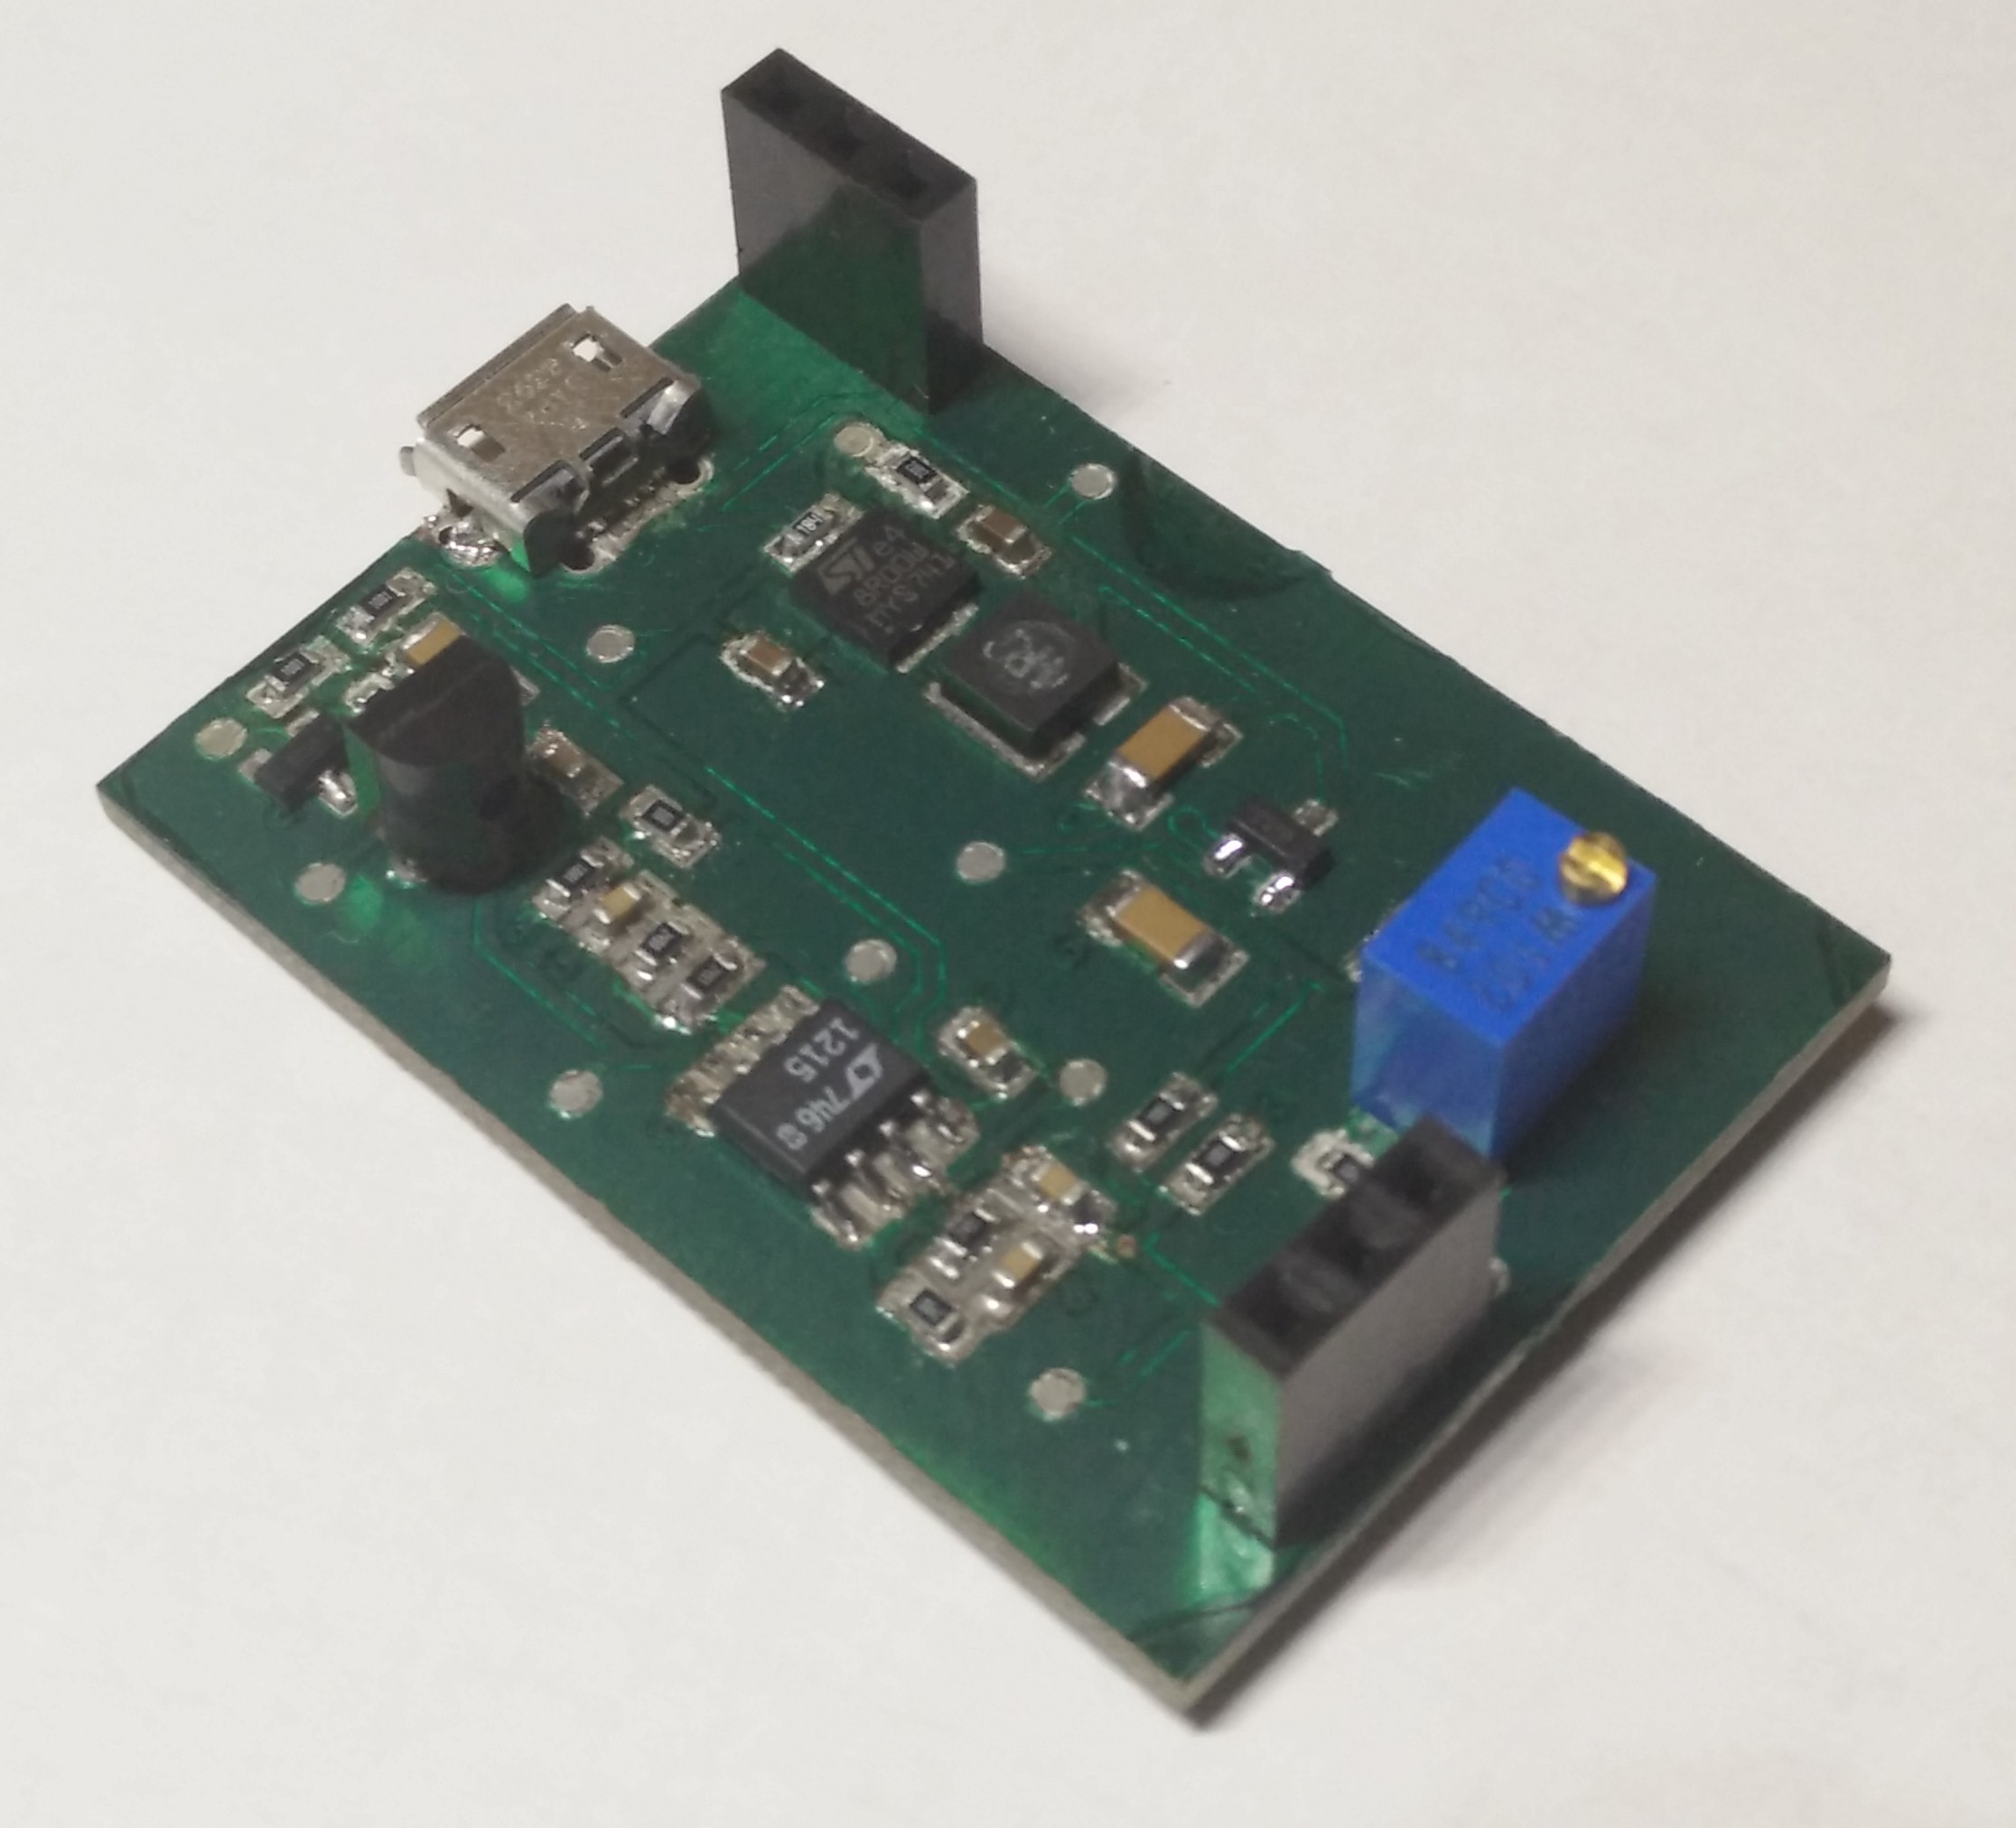
\includegraphics[width=0.6\textwidth]{fig/PCB_CROPPED.jpg}% TODO: fill in
      %   \caption{FFT of waveform shown in Figure \ref{fig:tp2_waveform}.}% TODO: replace with appropriate reference.
      %   \label{fig:tp2_fft}% TODO: update label with appropriate TP number
      % \end{figure}

        \begin{equation}
          V_{RMS} = 8.79mV.\nonumber
        \end{equation}

        \begin{figure}[H]
          \centering
          \subfloat[Time domain]{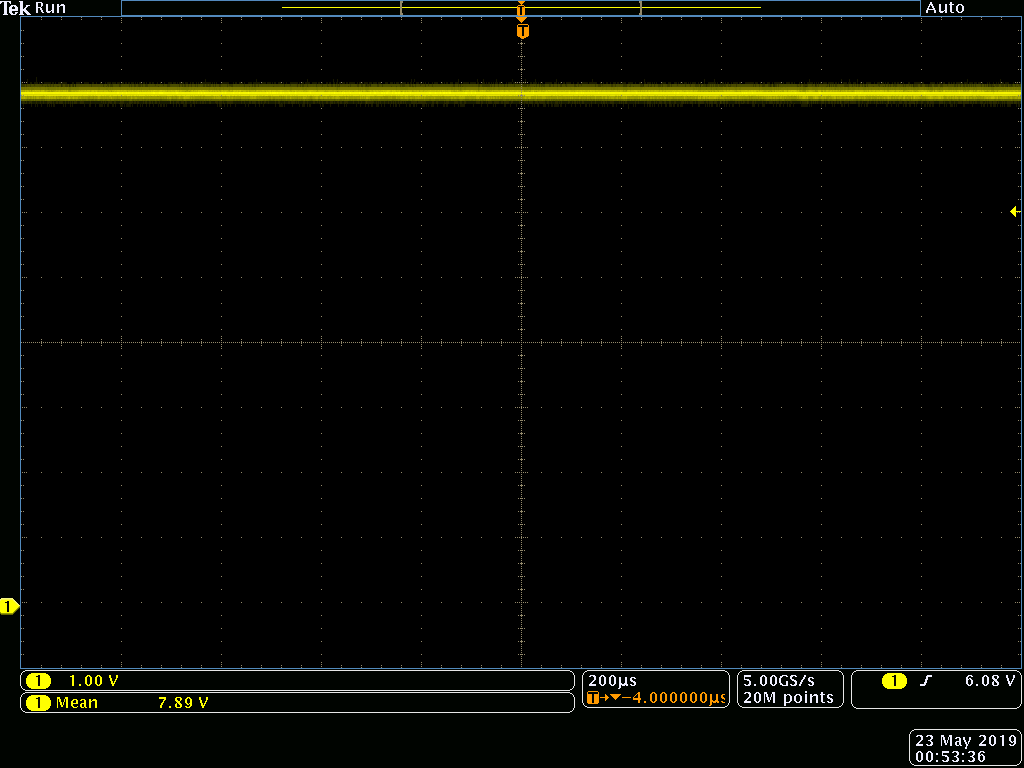
\includegraphics[width=0.65\textwidth]{fig/tp2_yt.png}}
          \qquad
          \subfloat[Frequency domain]{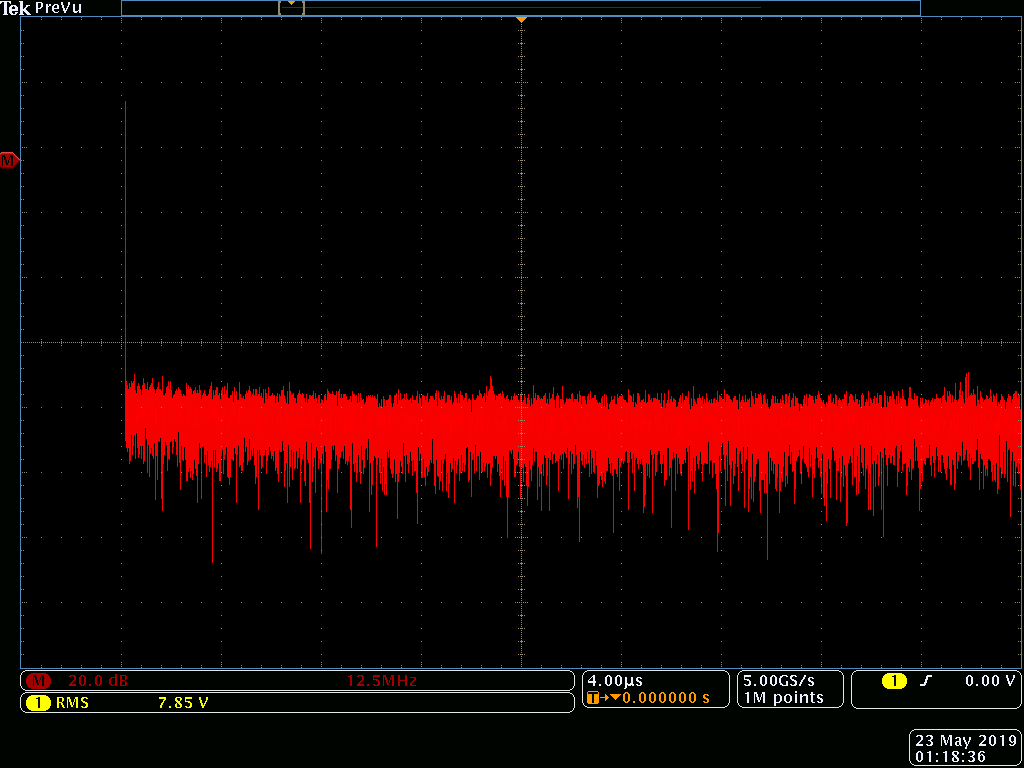
\includegraphics[width=0.65\textwidth]{fig/tp2_f_wide.png}}
          \caption{TP2}
          \label{fig:tp2_waveforms}
        \end{figure}
        \setcounter{subfigure}{0}


      \newpage
      \paragraph{TP4: Input to first op-amp}

        \begin{equation}
          V_{RMS} = 8.92mV.\nonumber
        \end{equation}

        \begin{figure}[H]
          \centering
          \subfloat[Time domain]{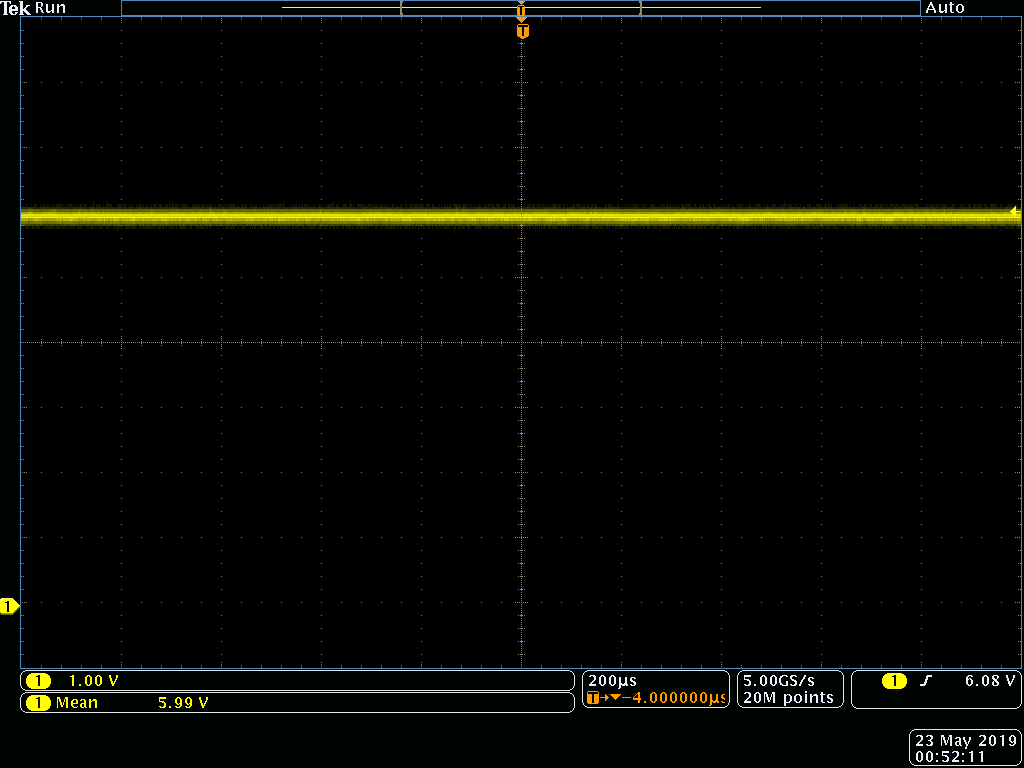
\includegraphics[width=0.7\textwidth]{fig/tp4_yt.png}}
          \qquad
          \subfloat[Frequency domain]{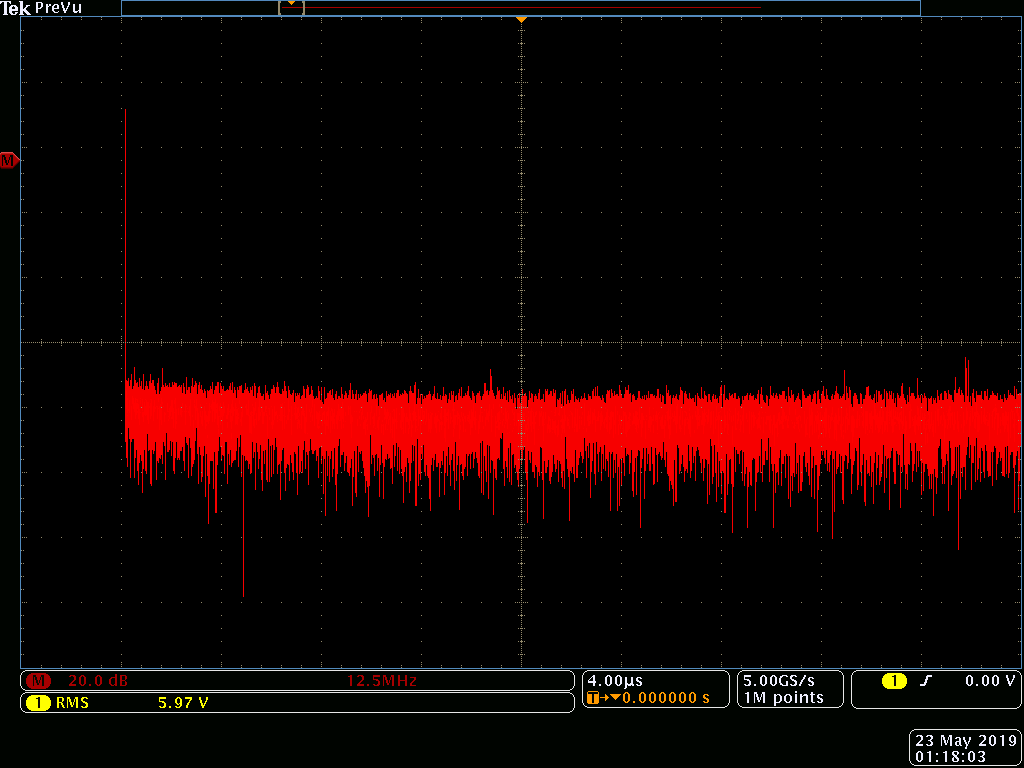
\includegraphics[width=0.7\textwidth]{fig/tp4_f_wide.png}}
          \caption{TP4}
          \label{fig:tp4_waveforms}
        \end{figure}
        \setcounter{subfigure}{0}

      \newpage
      \paragraph{TP8: Output of first op-amp/input to second op-amp}

        \begin{equation}
          V_{RMS} = 38.4mV.\nonumber
        \end{equation}

        \begin{figure}[H]
          \centering
          \subfloat[Time domain]{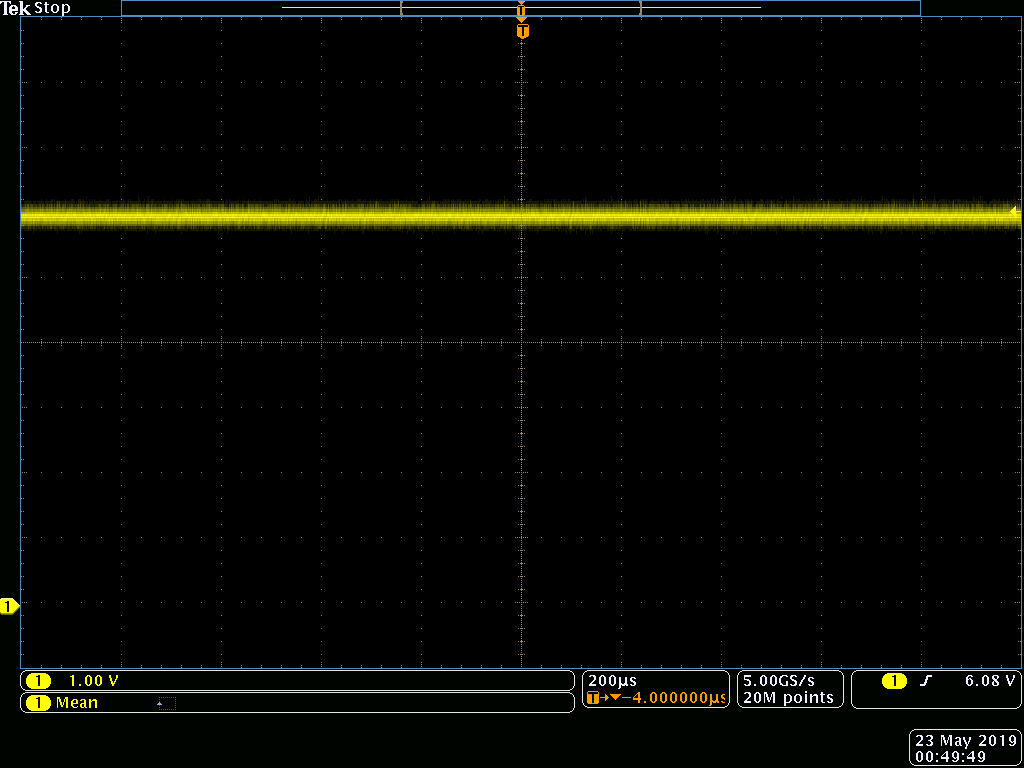
\includegraphics[width=0.7\textwidth]{fig/tp8_yt.png}}
          \qquad
          \subfloat[Frequency domain]{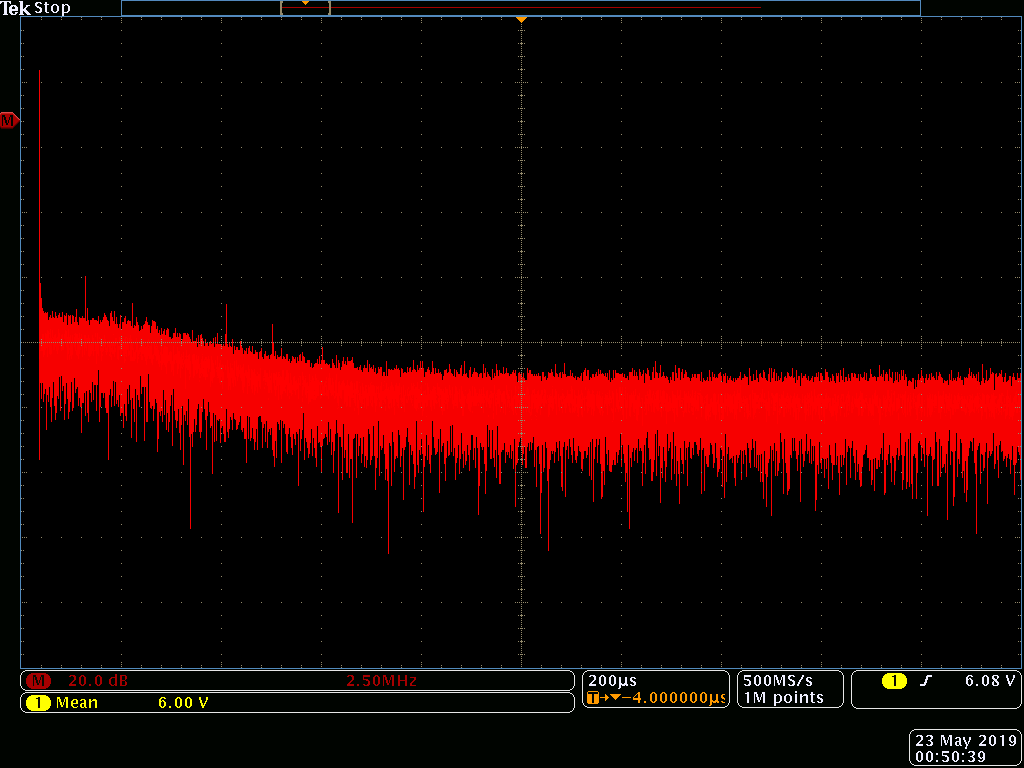
\includegraphics[width=0.7\textwidth]{fig/tp8_f.png}}
          \caption{TP8}
          \label{fig:tp8_waveforms}
        \end{figure}
        \setcounter{subfigure}{0}

      \newpage
      \paragraph{TP9: Output of second op-amp}

        \begin{equation}
          V_{RMS} = 363mV.\nonumber
        \end{equation}

        \begin{figure}[H]
          \centering
          \subfloat[Time domain]{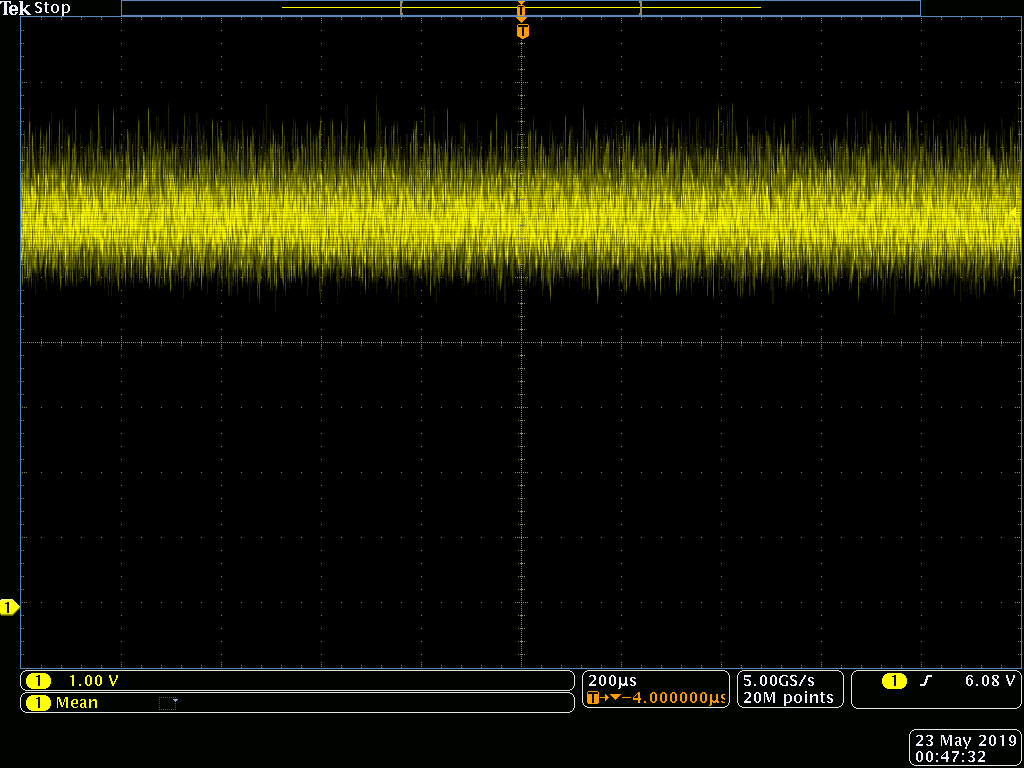
\includegraphics[width=0.7\textwidth]{fig/tp9_yt.png}}
          \qquad
          \subfloat[Frequency domain]{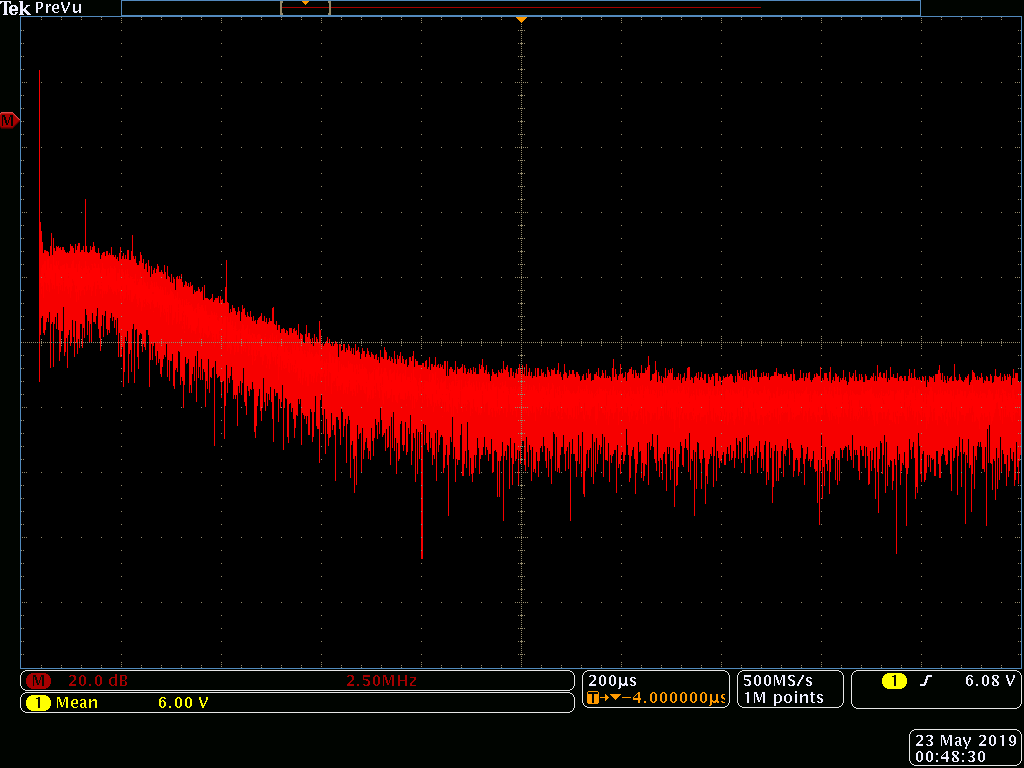
\includegraphics[width=0.7\textwidth]{fig/tp9_f.png}}
          \caption{TP9}
          \label{fig:tp9_waveforms}
        \end{figure}
        \setcounter{subfigure}{0}

      \newpage
      \paragraph{TP10: Circuit noise output}

        \begin{equation}
          V_{RMS} = 343mV.\nonumber
        \end{equation}

        \begin{figure}[H]
          \centering
          \subfloat[Time domain]{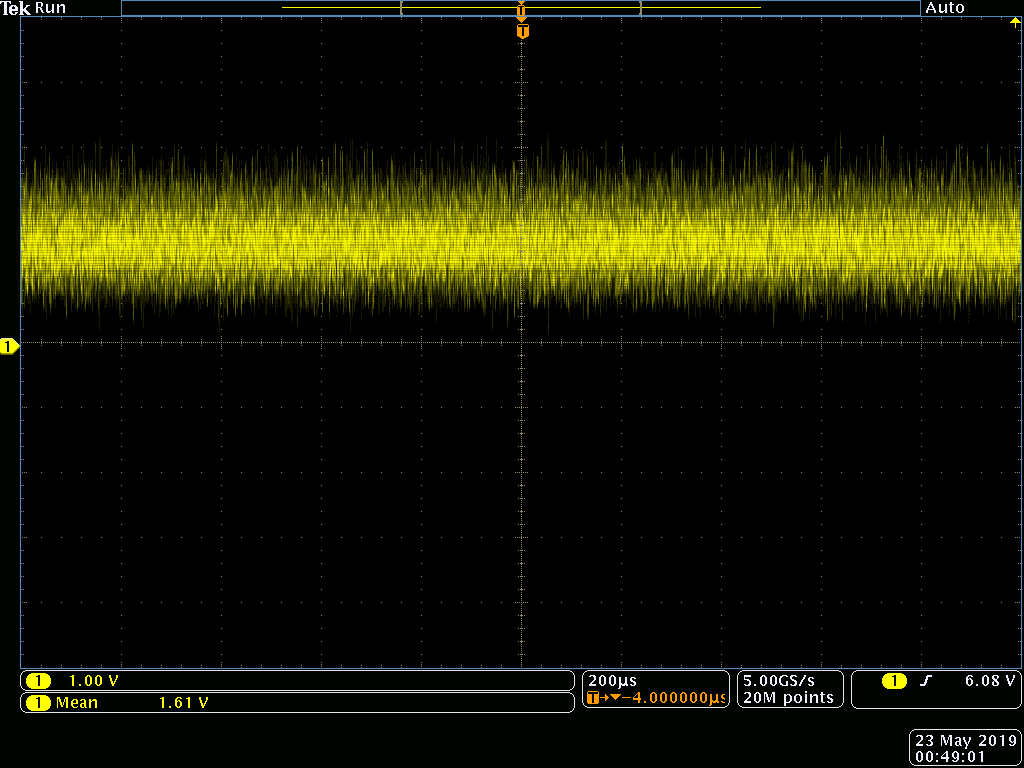
\includegraphics[width=0.7\textwidth]{fig/tp10_yt.png}}
          \qquad
          \subfloat[Frequency domain]{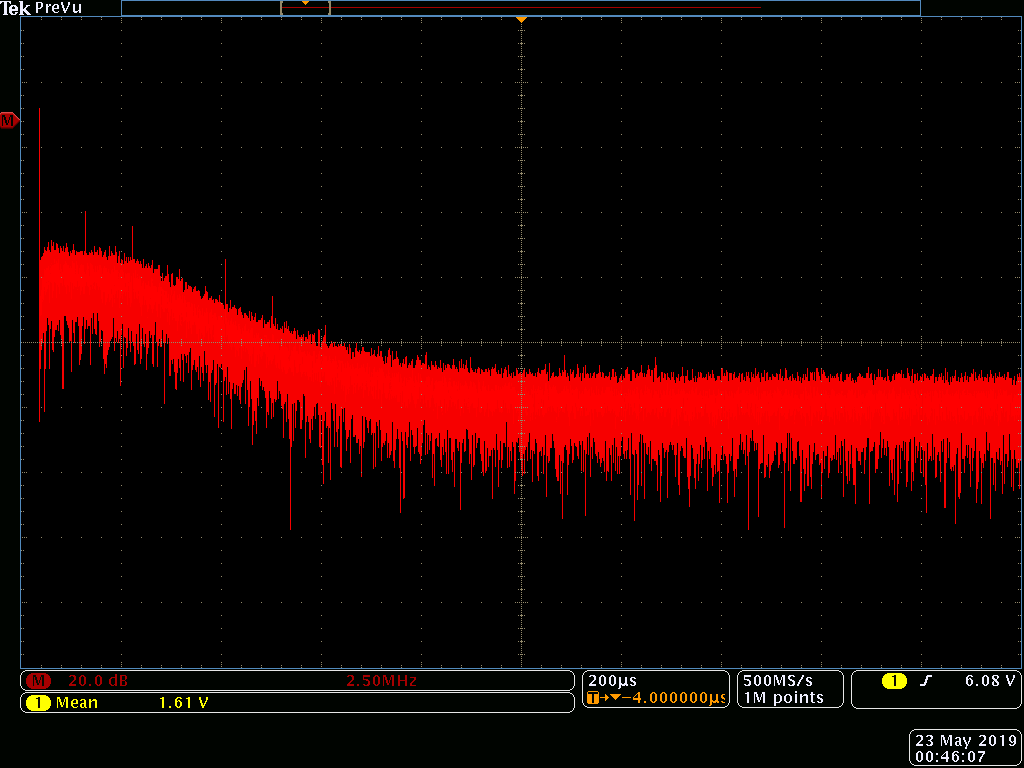
\includegraphics[width=0.7\textwidth]{fig/tp10_f.png}}
          \caption{TP10}
          \label{fig:tp10_waveforms}
        \end{figure}
        \setcounter{subfigure}{0}

    \subsubsection{Discussion}
      These measurements suggest that at lower frequencies, the circuit behaves as intended:
      \begin{itemize}
        \item From TP2 to TP4, the signal has similar $V_{RMS}$ whilst the DC bias voltage goes from 7.85V to 6V. This is expected since the signal has passed through an AC coupling capacitor, with a 6V bias set on the output side by a potential divider.
        \item The transition from TP4 to TP8 shows the effect of the first op-amp stage; $V_{RMS}$ increases whilst the DC bias voltage remains at 6V.
        \item The second op-amp stage lies between test points 8 and 9. Again $V_{RMS}$ increases whilst $V_{av}$ remains at 6V.
        \item Between TP9 and TP10, there is a final AC coupling stage to modulate the AC noise signal about a 1.65V DC voltage ($V_{cc}$/2 for connecting to one of the iCE40 comparator inputs). This appears to have little impact on $V_{RMS}$.
      \end{itemize}

      The frequency domain plots (Figures \ref{fig:tp8_waveforms} and \ref{fig:tp9_waveforms}) show that the op-amp gain falls to unity at around 10MHz --- this agrees with the plot of voltage gain vs frequency in the device's datasheet~\cite{lt1215}. The output $V_{RMS}$ unexpectedly appears much higher than the 100mV stated in The Art of Electronics~\cite[p.~984]{art_of_electronics}.

      % One problem identified during testing was the tendency for the 12V boost regulator's inductor to get very hot during operation; whilst the circuit still functions in a room temperature environment, a further prototype iteration would use an inductor with a higher current rating to improve reliability. This might require a redesign of the PCB to accommodate a larger inductor package and footprint, although similarly sized alternatives are available\footnote{e.g. Coilcraft XAL4030-472MEC with a 5.1A RMS current rating, compared to the 1.2A for the Wurth Elektronik 744031004 currently being used. The datasheet for the ST8R00 step-up regulator states an absolute maximum inductor current of 3A~\cite{ST8R00}.}.

  \subsection{Randomness Testing} \label{subsection:eval_randomness}
    The author used an improved version of the NIST Statistical Test Suite, developed by Cisco~\cite{arcetri_sts}, to assess the randomness of the bits produced when the hardware entropy source was connected to a comparator input on an iCE40 FPGA (on a Warp-FPGA board~\cite{stanley2018hardware}). The comparator output was sampled using a Digilent Analog Discovery 2, allowing 2 million random bits to be recorded (at 10kilobits per second, clocked by the iCE40's low frequency oscillator) for analysis.\\

    When running the test suite~\cite{nist_test_suite}, the input data is split into $i$ \textit{iterations} of length $S$ bits, where a greater $i$ value leads to a more accurate result\footnote{The accompanying NIST report~\cite{nist_test_suite} suggests at least 55 iterations.}, but also a smaller $S$ value for a given amount of sample data (which can prevent some tests from running; a recommended~\cite{arcetri_sts} $S$ value is $2^{20}$). Each test run as part of the suite consists of two \textit{analyses}; a test is said to have passed if:
    \begin{itemize}
      \item Proportion analysis: the proportion of the $i$ iterations which pass the test falls within a certain confidence interval.
      \item Uniformity analysis: the distribution of test P-values for each of the $i$ iterations is sufficiently uniformly distributed.
    \end{itemize}

    Different $i$, $S$ combinations were used to obtain the following results:

    \subsubsection{$i$ = 80, $S$ = 25000}
      The following tests were not run due to $S$ being too small: Rank, Overlapping Template, Universal, Approximate Entropy, Random Excursions, Random Excursions Variant, Serial, Linear Complexity.\\

      150/155 tests passed both analyses:
      \begin{table}[H]
        \centering
        \begin{tabular}{|c||c|c|}
          \hline
          Test Failed & Proportion & Uniformity\\
          \hline
          \hline
          Runs & X & \\
          \hline
          3/148 of Non-overlapping Template Matching & X & \\
          \hline
          1/148 of Non-overlapping Template Matching & X & X\\
          \hline
        \end{tabular}
        \caption{Tests failed when using a valid number of iterations. Failures are denoted by an X. }
        \label{table:nist_80}
      \end{table}

      \subsubsection{$i$ = 2, $S$ = 1000000}
        155/188 tests passed both analyses:
        \begin{table}[H]
          \centering
          \begin{tabular}{|c||c|c|}
            \hline
            Test Failed & Frequency & Proportion\\
            \hline
            \hline
            Frequency & X & \\
            \hline
            Cumulative Sums (forward) & X & \\
            \hline
            Cumulative Sums (backward) & X & \\
            \hline
            Runs & X & X\\
            \hline
            3/148 of Non-overlapping Template Matching & X & \\
            \hline
            8/8 of Random Excursions & X & X\\
            \hline
            18/18 of Random Excursions Variant & X & X\\
            \hline
          \end{tabular}
          \caption{Tests failed when using enough bits per iteration to run the entire test suite. Failures are denoted by an X.}
          \label{table:nist_2}
        \end{table}

        A detailed analysis of these results, and the mathematics behind the test suite, is beyond the scope of this report; the fact that the majority of tests appear to have passed suggests that the hardware entropy source is likely to be sufficient for the requirements of this project. Additionally, as $i$ (and hence test accuracy) increased, the proportion of tests passed increased.\\

        One area for further investigation would be to gather a larger sample of random bits ($\gtrsim 60$ Megabits\footnote{The Analog Discovery 2 can only record 10 million samples at a time, so such a measurement would require several samples to be taken and concatenated later for testing.}), both with and without the hardware entropy source attached to the FPGA. This would allow for comparison of test results, whilst a larger sample size would allow the entire test suite to  be run with a sufficient number of iterations. The speed at which the above data could be acquired was significantly limited by the low clock frequency used to clock the random bit generator --- the iCE40's 48MHz high frequency oscillator could be used instead to overcome this limitation, though it is likely that this frequency would have to be divided down to a few MHz or less to minimise edge distortion due to low bandwidth in PCB traces and flying wires leading to a logic analyser, as well as to reduce cross talk between wires.


  \subsection{Scaling of Logic Implementations} \label{subsection:scaling}
    \subsubsection{Method}
      This section presents the results of investigating the effect of random number generator bit width (the number of bits in the output) on the size and complexity of the resulting FPGA implementation. The author used Yosys, a program from the Project IceStorm~\cite{icestorm} toolchain, to synthesise Verilog RTL on a desktop computer\footnote{AMD Ryzen 5 2600X Six-Core Processor 3.60GHz, 16GB RAM.}. The terminal commands used are contained within the Makefiles in the URNG/RNG repositories, allowing these measurments to be repeated by running \texttt{make synthurng}/\texttt{make synthrng} within the appropriate repository (see Section \ref{subsection:GitHub} for a list of repositories). At the end of the synthesis process, yosys prints statistics for the resulting logic circuit  --- this information is displayed in Section \ref{subsubsection:scaling_results}.

    \subsubsection{Results} \label{subsubsection:scaling_results}
      The following tables are taken from Yosys' output. The table headings are described here~\cite{techlib}:
      \begin{itemize}
        \item Wires: The number of wires in the circuit where the multibit WIRE[X:0] counts as a single wire.
        \item Bits: The number of wire bits in the circuit where the multibit WIRE[X:0] consists of X+1 wire bits.
        \item CARRY: The number of logic cells used for their carry logic circuits (a combinational logic circuit useful for arithmetic operations).
        \item DFFE: The number of logic cells used as D flip-flops with clock enable input.
        \item DFFESR: The number of logic cells used as D flip-flops with clock enable and synchronous reset inputs.
        \item LUT4: The number of logic cells used as ROM 4 input look-up tables.
        \item U, S CPU Time: Time taken for synthesis to complete (user time, system time).
        \item Mem: Total RAM used by Yosys to synthesise design.
      \end{itemize}

      \begin{table}[H]
        \centering
        \begin{tabular}{|c||c|c|c|c|c|c|c|c|c|}
          \hline
          &
          \multicolumn{2}{|c|}{No. of Wires}
          &
          \multicolumn{4}{|c|}{No. of Cells}
          &
          \multicolumn{2}{|c|}{Synthesis}\\
          \hline
          N & Wires & Bits & CARRY & DFFE & DFFESR & LUT4 & U, S CPU Time/s & Mem/MB\\
          \hline
          \hline
          \textit{1} & \textit{29} & \textit{30} & \textit{0} & \textit{6} & \textit{4} & \textit{12} & \textit{0.27, 0.113} & \textit{28.93}\\
          \hline
          2 & 33 & 37 & 0 & 5 & 7 & 16 & 0.30, 0.05 & 29.00\\
          \hline
          \textit{3} & \textit{44} & \textit{58} & \textit{3} & \textit{6} & \textit{9} & \textit{25} & \textit{0.34, 0.08} & \textit{29.01}\\
          \hline
          4 & 41 & 56 & 1 & 7 & 10 & 24 & 0.34, 0.08 & 29.02\\
          \hline
          \textit{5} & \textit{49} & \textit{73} & \textit{5} & \textit{8} & \textit{12} & \textit{31} & \textit{0.33, 0.06} & \textit{29.04}\\
          \hline
          8 & 46 & 76 & 2 & 11 & 15 & 30 & 0.33, 0.17 & 35.29\\
          \hline
          16 & 60 & 117 & 3 & 19 & 24 & 45 & 0.52, 0.14 & 29.27\\
          \hline
          32 & 85 & 193 & 4 & 35 & 41 & 71 & 0.73, 0.19 & 29.55\\
          \hline
          64 & 119 & 326 & 5 & 67 & 74 & 106 & 1.14, 0.25 & 30.50\\
          \hline
        \end{tabular}
        \caption{Effect of varying uniform RNG bit width, BX, on logic circuit size. Odd numbered bit widths are printed in italics.}
        \label{table:urng_bx}
      \end{table}

      \begin{table}[H]
        \centering
        \begin{tabular}{|c||c|c|c|c|c|c|c|c|c|}
          \hline
          &
          \multicolumn{2}{|c|}{No. of Wires}
          &
          \multicolumn{4}{|c|}{No. of Cells}
          &
          \multicolumn{2}{|c|}{Synthesis}\\
          \hline
          N & Wires & Bits & CARRY & DFFE & DFFESR & LUT4 & U, S CPU Time/s & Mem/MB\\
          \hline
          \hline

          \hline
        \end{tabular}
        \caption{Effect of varying nonuniform RNG bit width, BY, on logic circuit size (for constant URNG bit width BX). Odd numbered bit widths are printed in italics.}
        \label{table:rng_by}
      \end{table}

      \begin{table}[H]
        \centering
        \begin{tabular}{|c||c|c|c|c|c|c|c|c|c|}
          \hline
          &
          \multicolumn{2}{|c|}{No. of Wires}
          &
          \multicolumn{4}{|c|}{No. of Cells}
          &
          \multicolumn{2}{|c|}{Synthesis}\\
          \hline
          N & Wires & Bits & CARRY & DFFE & DFFESR & LUT4 & U, S CPU Time/s & Mem/MB\\
          \hline
          \hline

          \hline
        \end{tabular}
        \caption{Effect of varying URNG bit width, BX, on RNG logic circuit size (for constant RNG output bit width BY). Odd numbered bit widths are printed in italics.}
        \label{table:rng_bx}
      \end{table}
    \subsubsection{Discussion}


    \textit{$\langle$ TODO: evaluate e.g. number of LUTs etc.$\rangle$}\\
    \textit{$\langle$ TODO: investigate how URNG and RNG logic implementations scale with various parameters (and how this compares to a naive implementation)$\rangle$}\\

    \textit{$\langle$ TODO: investigate scaling of adder hardware (inferred from Verilog vs iCE40 hardware accumulators)$\rangle$}
\newpage



%
% CONCLUSIONS
%

\section{Conclusions}

  The work done over the course of this project is contained within many different GitHub repositories, which can make it difficult to see how various pieces of work fit together. For a relatively small project such as this, it may have been simpler to keep all work within a single repository, though this would make it more difficult to reuse and/or modify individual components in future research/projects.

  \subsection{Future Work}
    The most obvious path for future work is to continue with the implemenatation of the system outlined above, in order to reduce a working prototype. As a research project, the characterisation work described in Section \ref{section:characterisation} was prioritised over working towards a working prototype, for the purposes of inspiring future research.\\

    One potential area for future research is the application of the Newton language to safeguarding against \textit{transduction attacks} (attacks on a computer system performed by manipulating transducers i.e. sensors in the system). This idea was briefly investigated by the author in parallel to this project, resulting in the publication of a poster~\cite{eurosys_poster} presented by the author at EuroSys 2019 in Dresden. The overall idea behind the poster was that Newton could be used to describe plausible system behaviour (e.g. constraints imposed by physical laws governing the system), thereby allowing implausible behaviour to be recognised and interpreted as a possible transduction attack in progress. The poster is summarised in Appendix \ref{poster_appendix}.


\newpage



\noindent

% Hack to remove REFERENCES REFERENCES header
\markboth{}{}
\printbibliography
\markboth{}{}

\newpage

\begin{appendix}

  %
  % RISK ASSESSMENT RETROSPECTIVE
  %

  \section{Risk Assessment Retrospective}
    The risk assessment submitted at the start of the project does not mention any specific hazards besides office (computer) work, since the project is predominately software/firmware based (all project hardware operated at low voltages i.e. 12V or less). No other hazards were encountered during the course of the project, since the random noise generator PCBs were manufactured by the Dyson Centre's Electronics Development Group. In retrospect, although not part of the initial project specification, the risk assessment could have anticipated the possibility of manufacturing PCBs for the project. The hazards associated with this activity include high temperatures (from a soldering iron/oven/hot air gun) as well as chemical hazards associated with solder, fume extraction etc.



  %
  % UPPER BOUND ON DIFF PRIV
  %

  \section{Derivation of an Upper Bound on \textit{Indirect} Differential Privacy Loss} \label{appendix:diff_priv_loss}
    Let $\hat{X}$ be a random variable denoting a sensor measurement, including any measurement error.
    \\
    \\
    Let $N_{Laplace}^\lambda$ be a random variable following a Laplace distribution with parameter $\lambda$. This represents random noise added to sensor measurements.
    \\
    \\
    Let $X$ be a random variable representing a \textit{noised} sensor measurement i.e. the masked value that the differential privacy system provides to the outside world after applying Laplace distributed noise to a measurement:
    \begin{equation}
      X = \hat{X} + N_{Laplace}^\lambda.
    \end{equation}
    A measurement event comprises the variable $\hat{X}$ taking on value $\hat{x}$. Similarly, a noising event can be defined by $X$ taking value $x = \hat{x} + n$. We define an embedded system as having $n$ sensors with measurements distributed as $\hat{X}_i$, $1 \leq i \leq n$.
    \\
    \\
    Let $Y$ denote a variable derived from one or more \textit{noised measurements}, $X$, such as measurements from different sensors in an embedded system:
    \begin{align*}
      Y & = f(X_1, X_2, ..., X_n) = f(\bf{X}),\\
      y & = f(x_{1}, x_{2}, ..., x_{n}) = f(\bf{x}).
    \end{align*}
    This same mapping function $f(\bf{x})$ can take unnoised measurements as arguments:
    \begin{align*}
      \hat{Y} & = f(\hat{X}_1, \hat{X}_2, ..., \hat{X}_n) = f(\bf{\hat{X}}),\\
      \hat{y} & = f(\hat{x}_{1}, \hat{x}_{2}, ..., \hat{x}_{n}) = f(\bf{\hat{x}}).
    \end{align*}
    Using this function, an untrusted party can compute an instance value $y$ by taking measurements $x_{1}$ to $x_{n}$ --- variable $\hat{Y}$ has experienced some privacy loss, $l_{\hat{Y}}$, since a noised instance value $y$ has effectively been released to the outside world (i.e. untrusted parties), revealing some information about the private noise-free value $\hat{y}$ taken by variable $\hat{Y}$. The privacy loss can be quantified using a log-likelihood ratio~\cite{Choi2018GuaranteeingLD} (Equation \ref{eqn:privacy_loss}). This privacy loss function requires two parameters,  $\hat{y}_a$ and $\hat{y}_b$, which are the possible \textit{true} i.e. noise-free values for $\hat{Y}$ that maximise the privacy loss (Equation \ref{eqn:argmax}).
    \begin{equation}
      y_{obs} = f(\bf{x}_{obs}) = \text{value for $y$ calculated from noised measurements $\bf{x}_i$}, \nonumber\\
    \end{equation}
    \begin{align}
      % \bf{\hat{x}_a}, \bf{\hat{x}_b} & = \argmax_{\bf{\hat{x}_a}, \bf{\hat{x}_b}} l_{\hat{Y}}(\bf{\hat{x}_a}, \bf{\hat{x}_b}) \label{eqn:argmax}\\
      % l_{\hat{Y}}(\bf{\hat{x}_a}, \bf{\hat{x}_b}) & = log \left( \frac{Pr\{ Y = y_{obs} | \bf{\hat{X}} = \bf{\hat{x}_a} \}}{Pr\{ Y = y_{obs} | \bf{\hat{X}} = \bf{\hat{x}_b} \}} \right) \label{eqn:privacy_loss}
      \hat{y}_a, \hat{y}_b & = \argmax_{\hat{y}_a, \hat{y}_b} l_{\hat{Y}}(\hat{y}_a, \hat{y}_b), \label{eqn:argmax}\\
      l_{\hat{Y}}(\hat{y}_a, \hat{y}_b) & = log \left( \frac{Pr\{ Y = y_{obs} | \hat{Y} = \hat{y}_a \}}{Pr\{ Y = y_{obs} | \hat{Y} = \hat{y}_b \}} \right). \label{eqn:privacy_loss}
    \end{align}
    Equation \ref{eqn:privacy_loss} can be rewritten as follows, where $\bf{\hat{x}_a}$ and $\bf{\hat{x}_b}$ are chosen to maximise $l_{\hat{Y}}$ as before, but subject to constraints $\bf{\hat{x}_a}$ $ = f^{-1}(\hat{y}_a)$ and $\bf{\hat{x}_b}$ $ = f^{-1}(\hat{y}_b)$:
    \begin{align}
      l_{\hat{Y}}(\bf{\hat{x}_a}, \bf{\hat{x}_b}) & = log \left( \frac{Pr\{ \bf{X} = \bf{x}_{obs} | \bf{\hat{X}} = \bf{\hat{x}_a} \}}{Pr\{ \bf{X} = \bf{x}_{obs} | \bf{\hat{X}} = \bf{\hat{x}_b} \}} \right). \label{eqn:exact_indirect_priv_loss}
    \end{align}
    This constrained optimisation problem could be solved to calculate an exact value for privacy loss. Alternatively, an upper bound on privacy loss can be determined using a far simpler calculation (the sum of privacy losses for each individual sensor):
    \begin{align}
      l_{\hat{Y}}(\bf{\hat{x}_a}, \bf{\hat{x}_b}) & = log \left( \prod_{u=1}^n \frac{Pr\{ X_u = x_{u,obs} | \hat{X}_u = \hat{x}_{u,a} \}} {Pr\{ X_u = x_{u,obs} | \hat{X}_u = \hat{x}_{u,b} \}} \right), \nonumber \\
      & \leq log \left( \prod_{u=1}^n \frac{Pr\{ X_u = x_{u,obs} | \hat{X}_u = \hat{x}_{u,c} \}}{Pr\{ X_u = x_{u,obs} | \hat{X}_u = \hat{x}_{u,d} \}} \right), \label{eqn:upper_bound} \\
      \text{where:} & \nonumber \\
      & \hat{x}_{u,c} = \argmax_{\hat{x}_{u,c}}Pr\{ X_u = x_{u,obs} | \hat{X}_u = \hat{x}_{u,c} \}, \nonumber \\
      & \hat{x}_{u,d} = \argmin_{\hat{x}_{u,d}}Pr\{ X_u = x_{u,obs} | \hat{X}_u = \hat{x}_{u,d} \}, \nonumber
    \end{align}
    i.e. the constraint $f^{-1}(\hat{y})$ has been removed. Equation \ref{eqn:upper_bound} can be interpreted as the sum of the privacy losses incurred by the $X$ variables i.e. $\sum_{u=1}^n l_{X_u}$. $Pr\{ X_u = x_{u,obs} | \hat{X}_u = \hat{x}_u \}$ is simply the Laplace distribution of the noise applied to the measurement represented by $\hat{X}$, centred on value $\hat{x}$.\\

    Note that this privacy loss is incurred when all values $x_{1,obs}$ to $x_{n,obs}$ are provided to the outside world (i.e. the event where an attacker transitions from having no information to the system to being provided with $x_{1,obs}$ to $x_{n,obs}$); for each subsequent individual query response $x_{u,obs}$, the resulting privacy loss is only:
    \begin{align}
      l_{\hat{Y}}(\bf{\hat{x}_a}, \bf{\hat{x}_b}) & = log \left( \frac{Pr\{ X_u = x_{u,obs} | \hat{X}_u = \hat{x}_{u,a} \}} {Pr\{ X_u = x_{u,obs} | \hat{X}_u = \hat{x}_{u,b} \}} \right),
    \end{align}
     where values for $\bf{\hat{x}_a}$ and $\bf{\hat{x}_b}$ are the same as those used in Equation \ref{eqn:exact_indirect_priv_loss} (if calculating exact privacy loss) or Equation \ref{eqn:upper_bound} (if calculating an upper bound).\\

    Since the Newton language recently gained a mutual information operator, the author attempted to factor mutual information into this calculation. Unfortunately, it appears that mutual information alone does not provide enough information to calculate indirect privacy loss --- the exact nature of the correlation between two (or more) random variables is required i.e. the conditional distribution for the unknown variable given known ones:
    \\
    \\
    Define $\hat{X}$ and $X$ as before and let $\hat{Y}$ be a random variable correlated with $\hat{X}$. Both $\hat{X}$ and $\hat{Y}$ can take values within some range (e.g. due to finite sensor precision):
    \begin{align*}
      \hat{X} \in R_{\hat{X}},\ \hat{Y} \in R_{\hat{Y}},
    \end{align*}
    The mutual information $I(\hat{X};\hat{Y})$ is defined as:
    \begin{align}
      I(\hat{X};\hat{Y}) = \int_{R_{\hat{Y}}} \int_{R_{\hat{X}}} p(\hat{X}, \hat{Y}) log \left( \frac{p(\hat{X}, \hat{Y})}{p(\hat{X})p(\hat{Y})} \right) d\hat{X} d\hat{Y},
    \end{align}
    where $p()$ denotes the probability density function for a random variable. The author has been unable to insert this value into the privacy loss equation, however a value for privacy loss can be obtained if the conditional distribution of $\hat{X}$ given $\hat{Y}$ is known, as this allows the conditional distribution of $X$ given $\hat{Y}$ to be calculated:
    \begin{equation}
      Pr\{X = x | \hat{Y} = \hat{y}\} = \int_{R_{\hat{X}}}Pr\{X = x | \hat{X} = \hat{x}\} Pr\{\hat{X} = \hat{x} | \hat{Y} = \hat{y}\} d \hat{x} \label{eqn:p_x_given_y_hat}.
    \end{equation}
    Equation \ref{eqn:p_x_given_y_hat} can be substituted into Equation \ref{eqn:priv_loss_y_hat_initial}, the formula for privacy loss incurred by $\hat{Y}$ as a result of observing a value $x_{obs}$ for $X$. This results in Equation \ref{eqn:priv_loss_y_hat_final}:

    \begin{align}
      l_{\hat{Y}}(\hat{y}_a, \hat{y}_b) & = log \left( \frac{Pr\{X = x_{obs} | \hat{Y} = \hat{y}_a\}}{Pr\{X = x_{obs} | \hat{Y} = \hat{y}_b\}} \right) \label{eqn:priv_loss_y_hat_initial} \\
      & = log \left( \frac{\int_{R_{\hat{X}}} Pr\{X = x_{obs}| \hat{X} = \hat{x}\} Pr\{\hat{X}=\hat{x}|\hat{Y} = \hat{y}_a\} d\hat{x} }{\int_{R_{\hat{X}}} Pr\{X = x_{obs}| \hat{X} = \hat{x}\} Pr\{\hat{X}=\hat{x}|\hat{Y} = \hat{y}_b\} d\hat{x} }\right) \label{eqn:priv_loss_y_hat_final},
    \end{align}
    for $\hat{y}_a, \hat{y}_b = \argmax_{\hat{y}_a, \hat{y}_b}(l_{\hat{Y}})$ as before.
  %
  % NOISE GENERATOR SCHEMATIC AND PCB LAYOUT
  %
  \newpage
  \section{Hardware Entropy Source Schematic and PCB} \label{appendix:schematic}
  \vspace{-1cm}
    \begin{figure}[H]
      \centering
      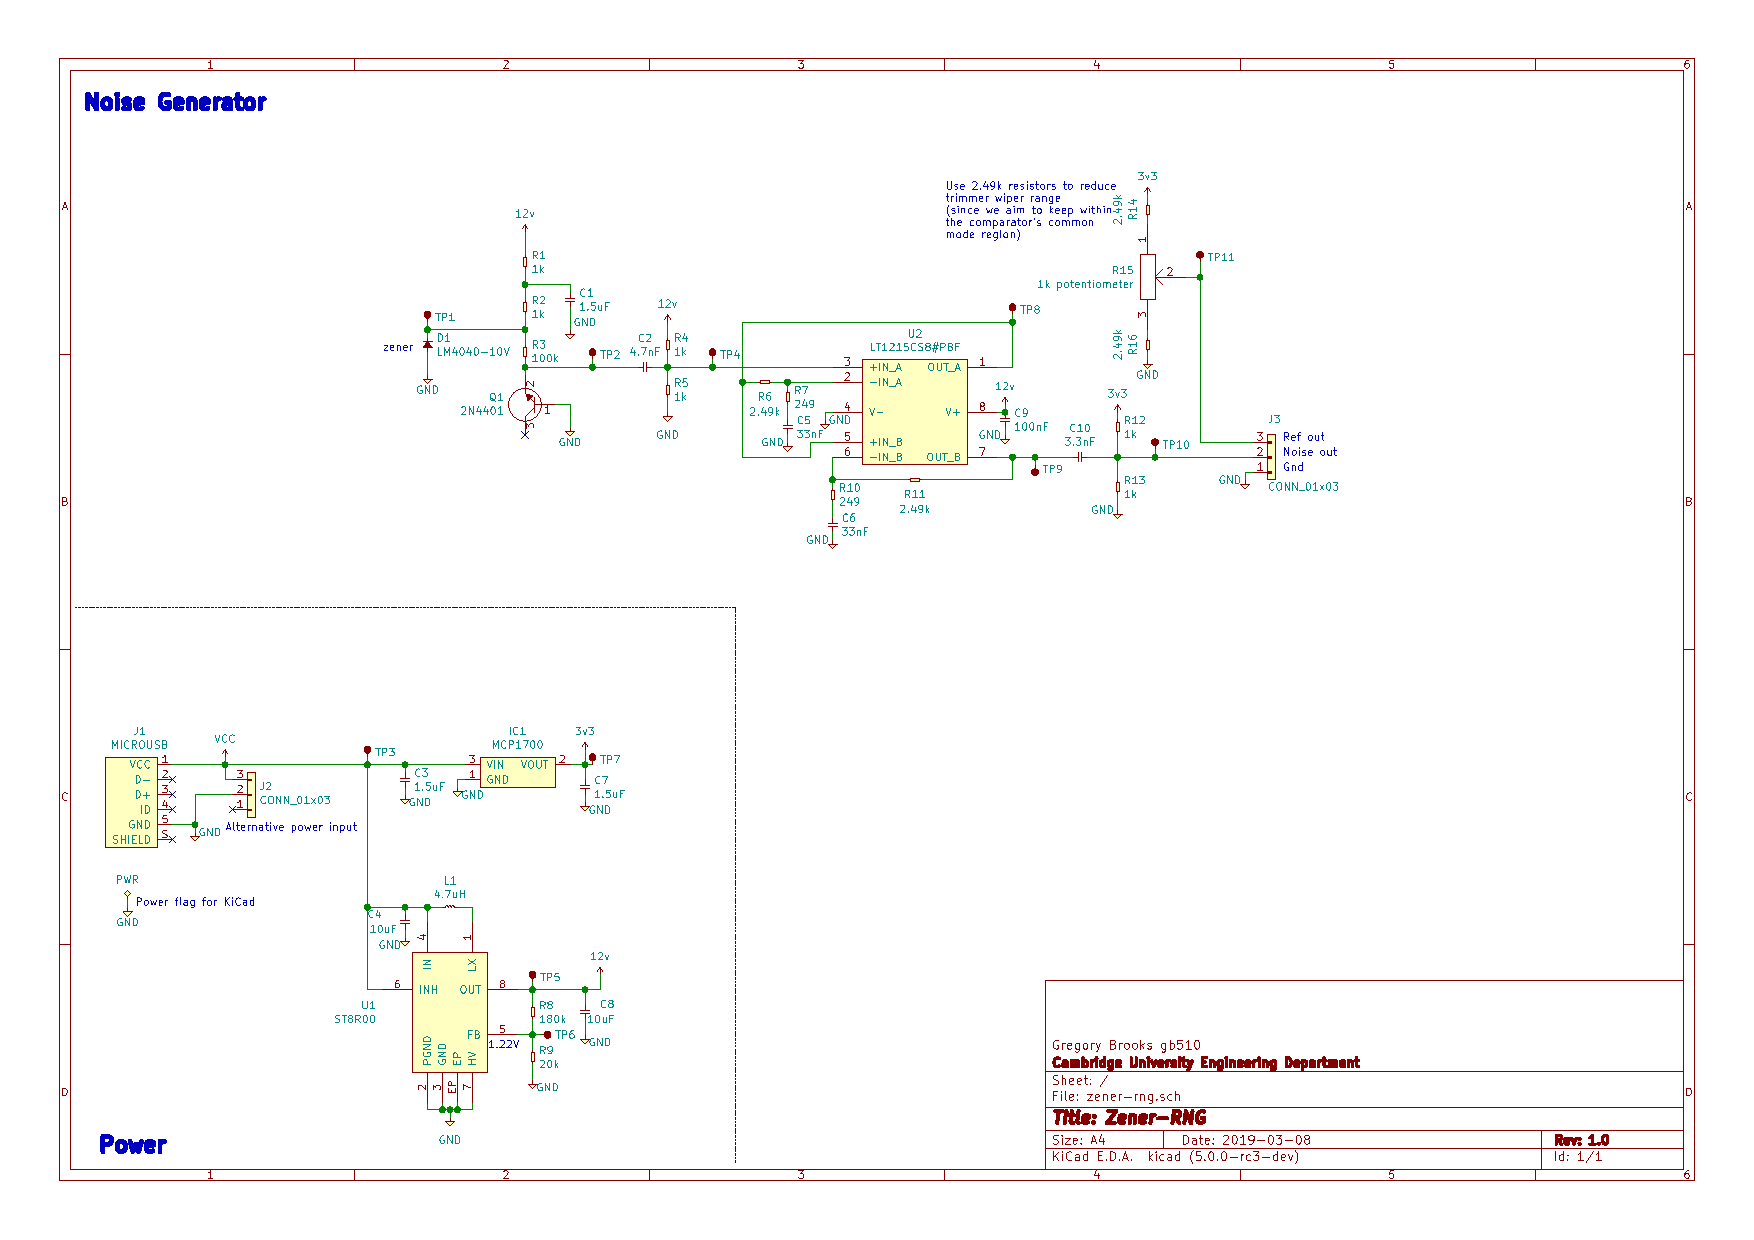
\includegraphics[angle=90,width=0.9\textwidth]{fig/schematic.pdf}
      \label{fig:schematic}
    \end{figure}

    \newpage

    \vspace{-1.5cm}
    \begin{figure}[H]
      \centering
      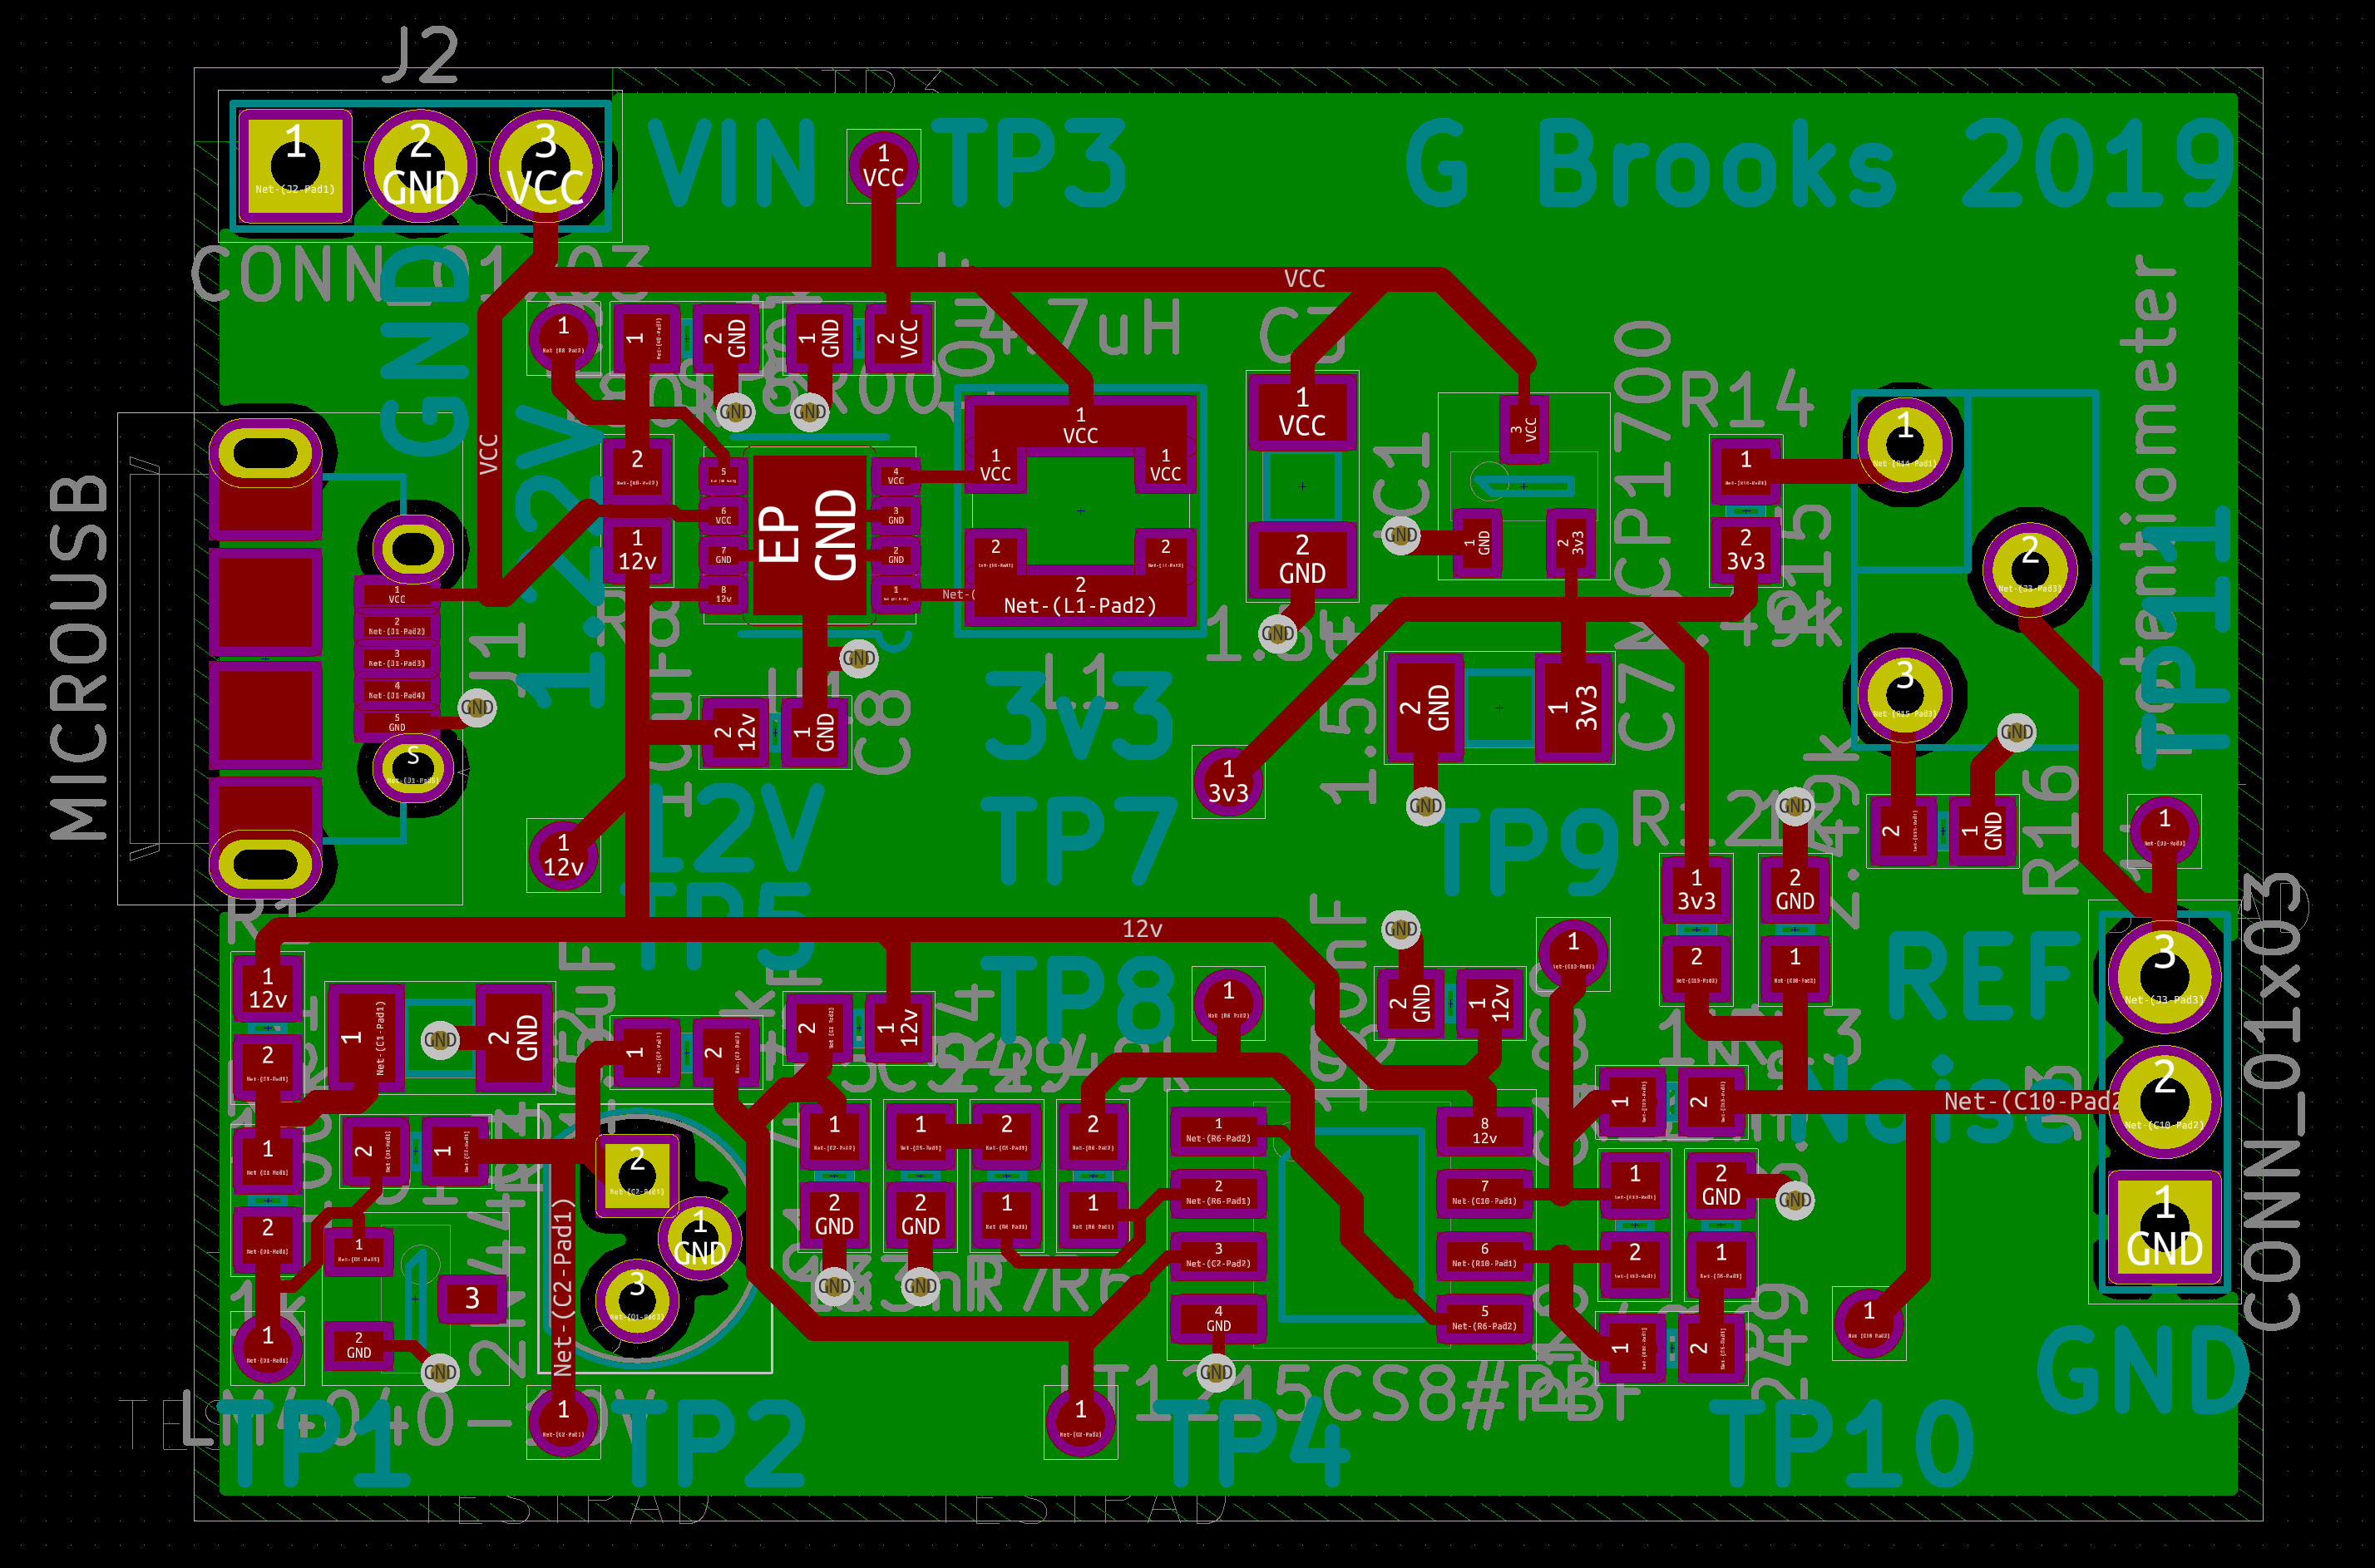
\includegraphics[angle=90, width=0.9\textwidth]{fig/pcb.PNG}
      \label{fig:pcb}
    \end{figure}

    \newpage

  %
  % EUROSYS POSTER
  %

  \section{EuroSys 2019 Poster: Safeguarding Sensor Device Drivers Using Physical Constraints} \label{poster_appendix}
    This poster~\cite{eurosys_poster} was submitted to EuroSys 2019, to communicate the idea of using information about a physical system to condition electronic sensor measurements. The example discussed in the poster is the detection and safeguarding against transduction attacks~\cite{Fu_2018}, where an attacker manipulates a sensor's output to gain control over a system. For example, research by Liu, Yan and Xu~\cite{autonomous_vehicles} has shown that the proximity sensors on a Tesla automobile can be fooled into providing erroneous (or even no) data using ultrasonic interference produced by a device built using off-the-shelf electronic components. An attacker is able to influence the system's behaviour without needing to directly manipulate the execution of the vehicle's firmware.\\

    The poster illustrates how the Newton language can be used to describe a physical system, in this case an accelerometer mounted to a PCB without vibration isolation. In this scenario, vibrations of the PCB (e.g. due to a nearby loudspeaker or even, in the case of a smartphone, due to loudspeakers mounted to the PCB) are measured by the accelerometer, obscuring a \textit{true} acceleration measurement i.e. acceleration of the entire system due to gravity. This effect is particularly pronounced if the board is driven at its resonant frequency, since the resulting oscillation will have a greater amplitude~\cite{adi}. This phenomenon could, in theory, be used as part of a transduction attack e.g. where a smartphone's loudspeaker is used to interfere with a software application's estimate of the device's physical orientation.\\

    To test whether this phenomenon can be distinguished from regular measurement noise, the author performed an experiment~\cite{poster_experiment} using an MMA8451Q accelerometer mounted on an FRDM-KL03Z board. With the sensor resting stationary on a horizontal surface, five minutes worth of accelerometer samples were recorded at 10Hz in order to obtain a probability distribution for the accelerometer's measurement noise (along the z axis, aligned with the vertical); this data was empirically observed to fit a Laplace distribution. This measurement was then repeated with the board resting on top of a smartphone playing a 440Hz audio tone --- in theory, this data (random samples from a sinusoid) would fit a bimodal beta distribution (see section \ref{Poster_Derivation} for derivation) allowing a log likelihood ratio to be computed:

    \begin{equation}
      LLR = -2 \sum_{i = 1}^{N} \frac{\frac{1}{\pi}\left| \frac{1}{\sqrt{A^2\omega^4 - \ddot{x}_i^2}} \right|}{\frac{1}{2b} exp\left(-\frac{|\ddot{x}_i-\mu|}{b}\right)}
    \end{equation}

    The value of this log-likelihood ratio indicates whether the audio tone based transduction attack described here is likely to be occuring. For the data collected in the experiment, the log-likelihood ratio was found to be around -24600.08 whilst the tone was playing, and +3731 when it was not; the negative value indicates that the measurements taken whilst the tone was playing were indeed more accurately described by the bimodal beta distribution, compared to the Laplace distribution of sensor noise, and vice versa for the positive value.

    \subsection{Derivation of Bimodal Beta Distribution} \label{Poster_Derivation}
    Let T be a uniformly distributed random variable representing the time at which acceleration is sampled:
    \begin{align}
      T & \sim U\left(-\frac{\pi}{\omega}, \frac{\pi}{\omega}\right), \nonumber \\
      f_T(t) & =
        \begin{cases}
          \frac{\omega}{2\pi} & -\frac{\pi}{\omega} \leq t \leq \frac{\pi}{\omega}\\
          0 & \text{otherwise}
        \end{cases},\\
      F_T(t) & =
        \begin{cases}
          0 & t < -\frac{\pi}{\omega}\\
          \frac{\omega (t + \pi / \omega)}{2\pi} & -\frac{\pi}{\omega} \leq t \leq \frac{\pi}{\omega}\\
          1 & t > \frac{\pi}{\omega}.
        \end{cases}.
    \end{align}
    Then let X = g(T) represent the acceleration value at time T. By considering the dynamics of the system, we know that:

    \begin{equation}
      g(t) = A \omega^2 sin(\omega t),
    \end{equation}
    where A is a frequency-dependent constant equal to the product of quality factor and board displacement at resonance. We can also define a monotonically increasing function $h(x)$ as the inverse of $g(t)$:

    \begin{equation}
      h(x) = g^{-1}(x) = \frac{1}{\omega} arcsin \left(\frac{x}{A\omega^2}\right).
    \end{equation}
    \\
    The cumulative distribution function for X can therefore be written in terms of the cumulative distribution function for T, accounting for the fact that g(t) is not monotonic:
    \begin{equation}
      F_X(x) = F_T(h(x)) + \Big(1 - F_T(\pi/\omega - h(x))\Big).
    \end{equation}
    \\
    Taking the derivative results in the probability density function for X:
    \begin{align}
      f_X(x) & = \Big(f_T(h(x) - f_T(-h(x)))\Big) \frac{d(h(x))}{dx}\\
      & =
      \begin{cases}
        \frac{1}{\pi \sqrt{A^2 \omega^4 - x^2}} & |x| \leq A \omega^2\\
        0 & \text{otherwise}
      \end{cases}.
    \end{align}

\end{appendix}

\end{document}
